\newcommand{\name}{Author}
\newcommand{\subtitel}{{Evaluation der Einsatzmöglichkeiten ausgewählter Machine-Learning-Verfahren im Kontext von IT-Governance-Prozessen, insbesondere im Application-Portfolio-Management}}
\newcommand{\titel}{Master-Thesis}
\newcommand{\strasse}{Adress}
\newcommand{\plz}{Adress}
\newcommand{\email}{Mail}
\newcommand{\matrikel}{wayne}
\newcommand{\semester}{Semester}
\newcommand{\abgabe}{28.12.2020}

\newcommand{\pdftitle}{Master-Thesis}
\newcommand{\pdfsubject}{Master-Thesis}
\newcommand{\pdfauthor}{\name}
\newcommand{\pdfkeywords}{keywords}

\newcommand{\vg}{vgl.}

\documentclass[
fontsize=12pt,
paper=a4,
ngerman,
DIV=calc,
oneside, %twoside
numbers=enddot,
headsepline,
listof=totoc,
bibliography=totoc,
index=totoc,
pointlessnumbers,
draft=false, 
parskip=full-,
BCOR=5mm %TODO
]{scrbook} %scrreprt, scrbook

\RedeclareSectionCommand[
  beforeskip=0pt,
  afterindent=false% <- added
  ]{chapter}

\clubpenalty = 10000
\widowpenalty = 10000 
\displaywidowpenalty = 10000

\usepackage[hyphens]{url}
\usepackage{multirow}
\usepackage[table,xcdraw]{xcolor}

\usepackage{enumitem}
\setlist{nosep}


\usepackage[ngerman]{babel}
\usepackage[T1]{fontenc}

%\usepackage{lmodern}       %Schriftart 
\usepackage{pslatex}

\usepackage{textcomp} % Euro-Zeichen etc.
\usepackage{microtype}
\usepackage[utf8]{inputenc}
\usepackage[paper=a4paper,left=35mm,right=25mm,top=20mm,bottom=20mm,includeheadfoot]{geometry}
\setlength{\footskip}{2cm} 

\usepackage[bookmarksdepth=subsection,colorlinks=false,pdfborder={0 0 0},plainpages=false]{hyperref}
%fuer hyperlinks im pdf-format
%PDF-META
\hypersetup{
 pdftitle={\pdftitle},
    pdfsubject={\pdfsubject},
    pdfauthor={\pdfauthor},
    pdfkeywords={\pdfkeywords}
  }


\usepackage{csquotes}


%\usepackage[round]{natbib}


%(\RequirePackage[ngerman=ngerman-x-latest]{hyphsubst}) Silbentrennung ggf

%Zitieren
\usepackage[
backend=biber,
%style=alphabetic,    % Zitierstil
bibstyle=numeric,
citestyle=numeric,
isbn=false,                % ISBN nicht anzeigen, gleiches geht mit nahezu allen anderen Feldern
url=true,
doi=false,
pagetracker=true,          % ebd. bei wiederholten Angaben (false=ausgeschaltet, page=Seite, spread=Doppelseite, true=automatisch)
maxbibnames=10,            % maximale Namen, die im Literaturverzeichnis angezeigt werden 
maxcitenames=4,            % maximale Namen, die im Text angezeigt werden, ab 3 wird u.a. nach den ersten Autor angezeigt
autocite=inline,           % regelt Aussehen für \autocite (inline=\parancite)
block=space,               % kleiner horizontaler Platz zwischen den Feldern
backref=false,              % Seiten anzeigen, auf denen die Referenz vorkommt
backrefstyle=three+,       % fasst Seiten zusammen, z.B. S. 2f, 6ff, 7-10
date=short,                % Datumsformat
%natbib=true,
bibencoding=utf8,
%firstinits=true, %depr given
giveninits=true,
%uniquename=init,
uniquename=false,
%dashed=false,
  clearlang=true
]{biblatex}

\AtEveryBibitem{%
  \clearlist{language}%
}

%%%%%%%%%%%%%%%%%%%%%%%%%%
%% Abkürzungsverzeichnis
%%%%%%%%%%%%%%%%%%%%%%%%%%
\usepackage[intoc,german]{nomencl}
\renewcommand{\nomname}{Abkürzungsverzeichnis}
\let\abk\nomenclature
\setlength{\nomlabelwidth}{.20\hsize}
\renewcommand{\nomlabel}[1]{#1 \dotfill}
\setlength{\nomitemsep}{-\parsep}
\makenomenclature

\usepackage{verbatim}

\usepackage{setspace}

%\usepackage{scrpage2}
%\usepackage[automark,footsepline,plainfootsepline,headsepline]{scrpage2} 
\usepackage[automark,headsepline]{scrpage2} 

%\automark[section]{chapter} 
%\usepackage{scrpage2} 



\renewcommand*{\finalnamedelim}{%
  \ifnumgreater{\value{liststop}}{2}{\finalandcomma}{}%
  \addspace\&\space}

\DefineBibliographyStrings{ngerman}{ 
   andothers = {{et\,al\adddot}},             
} 
 
 \renewcommand*{\nameyeardelim}{\addcomma\space}

\usepackage{xargs}                      % Use more than one optional parameter in a new commands

\usepackage[colorinlistoftodos,prependcaption,textsize=tiny]{todonotes}
\newcommandx{\unsure}[2][1=]{\todo[linecolor=red,backgroundcolor=red!25,bordercolor=red,#1]{#2}}
\newcommandx{\change}[2][1=]{\todo[linecolor=blue,backgroundcolor=blue!25,bordercolor=blue,#1]{#2}}
\newcommandx{\info}[2][1=]{\todo[linecolor=green,backgroundcolor=green!25,bordercolor=green,#1]{#2}}
\newcommandx{\improvement}[2][1=]{\todo[linecolor=purple,backgroundcolor=purple!25,bordercolor=purple,#1]{#2}}

\usepackage{array}

\newcolumntype{P}[1]{>{\hspace{0pt}}p{#1}}
\usepackage{rotating}



%Für hübsche Zitate
\usepackage{epigraph}

% \epigraphsize{\small}% Default
\setlength\epigraphwidth{13cm}
\setlength\epigraphrule{0pt}

\usepackage{etoolbox}

\makeatletter
\patchcmd{\epigraph}{\@epitext{#1}}{\itshape\@epitext{#1}}{}{}
\makeatother

\usepackage{booktabs}



%%%%Testweise

\addbibresource{literatur.bib}

%\addbibresource{internet.bib}


\begin{document}
\pagenumbering{alph}

	%\titlehead{FernUniversität in Hagen}

%\setkomafont{publishers}{\normalfont\sffamily}
%\setkomafont{author}{\normalfont\sffamily}
\setkomafont{publishers}{\large}
\setkomafont{author}{\large}
%\setkomafont{author}{\fontsize{12bp}}
%\setkomafont{author}{\fontsize{18bp}{20.8bp}} 


\subject{Frankfurt University of Applied Sciences}
\subtitle{\subtitel\\[2ex]}
\title{\titel\\[2ex]}
\author{zur Erlangung des akademischen Grades Master of Science (M. Sc.) \\
Studiengang Wirtschaftsinformatik\\
Fachbereich 2: Informatik und Ingenieurwissenschaften\\
[1.7ex]}
\publishers{
\begin{tabular}[t]{ll} 
Von:& 		\name\\ 
 	&	\strasse\\ 
 	&	\plz\\ 
E-Mail:& \email\\
Matrikelnummer:& \matrikel\\[2ex]

Gutachter:&	Univ.-Prof. Dr. Xyz\\ 
Betreuer:&	Dr. Xyz\\
\vspace{1cm}

Abgabe am:&	\abgabe\\ 
\end{tabular}

\vspace{1cm}
}
\date{}%Definitionen Titelblatt
\maketitle

\singlespacing


\pagenumbering{Roman}   % I, II, III... roman => i, ii, iii
\setcounter{page}{1}

\cleardoublepage

\pagestyle{plain}

\chapter*{Vorwort}
\addcontentsline{toc}{chapter}{Vorwort}  
Die vorliegende Master-Thesis wurde in Kooperation mit der Dangelmayer \& Seemann GmbH (Abk.: DS) erstellt. Die Problemstellung der Arbeit stammte von einem Kunden von DS. Es handelte sich bei dem Kunden um ein multinationales Großunternehmen. DS betreute das Unternehmen in beratender Funktion. Auf die Nennung von Details zum Unternehmen wird verzichtet. Es werden in dieser Arbeit keine vertraulichen Daten veröffentlicht, die einen Rückschluss auf das Unternehmen zulassen würden. Das Vorwort soll neben der Kurzbeschreibung des Umfelds auch für eine Danksagung genutzt werden: Ich bedanke mich herzlich bei allen Mitarbeitern der Dangelmayer \& Seemann GmbH, insbesondere bei Olaf Seemann, Dr. Wolf Pfannenstiel, Dr. Nedialka Bubner, sowie bei Andrew Smart für die Unterstützung während der Bearbeitungszeit. 
%\chapter*{Abstract}
\addcontentsline{toc}{chapter}{Abstract}  
test

\chapter*{Zusammenfassung}
\addcontentsline{toc}{chapter}{Zusammenfassung}  
test



\tableofcontents			%Inhaltsverzeichnis
\cleardoublepage

%Abstände checken
\listoffigures					% Abbildungsverzeichnis
\cleardoublepage
\listoftables					% Tabellenverzeichnis 
\cleardoublepage
%% Abkürzungsverzeichnis


	\abk{IT}{Informationstechnologie}
	\abk{B2B}{Business-to-Business}
	\abk{B2C}{Business-to-Customer}
	\abk{C2C}{Customer-to-Customer}
	\abk{P2P}{Peer-to-Peer}
	\abk{IT}{Informationstechnologie}
	\abk{IT}{Informationstechnologie}
	\abk{App}{Applikation}
	\abk{API}{Schnittstelle}
	\abk{ERP}{Enterprise-Resource-Planning}
	\abk{IKT}{Informations- und Kommunikationstechnologien}
	\abk{AS}{Anwendungssystem}
	\abk{EUR}{Euro}
	\abk{PFM}{Personal Financial Management}
	

%\clearpage
\markright{Abkürzungsverzeichnis}
%% Abstand vom linken Rand
\printnomenclature[2.9cm]
%\clearpage						% Abkürzungsverzeichnis
\cleardoublepage
\cleardoublepage

\pagenumbering{arabic}
\setcounter{page}{1}


%\renewcommand{\chapterpagestyle}{scrheadings}
\pagestyle{scrheadings}
%\clearscrheadings	
%\clearscrheadfoot
\automark[section]{chapter}

\ohead{}
\ihead{\headmark}
\chead{}
%\cfoot{\pagemark}

%%%%%%%%%%%%%%%%%%%%%%%%%%%%%%%%%BEGIN - Content
\onehalfspacing 
\clearpage



\chapter{Einleitung}
\label{einleitung}


\epigraph{e.g. Zitat}{--- \textup{Sebastian Wayne}, 2018}


Lorem \cite[]{Statista} ipsum dolor sit amet, consetetur sadipscing elitr, sed diam nonumy eirmod tempor invidunt ut labore et dolore magna aliquyam erat, sed diam voluptua. At vero eos et accusam et justo duo dolores et ea rebum. Stet clita kasd gubergren, no sea takimata sanctus est Lorem ipsum dolor sit amet. Lorem ipsum dolor sit amet, consetetur sadipscing elitr, sed diam nonumy eirmod tempor invidunt ut labore et dolore magna aliquyam erat, sed diam voluptua. At vero eos et accusam et justo duo dolores et ea rebum. Stet clita kasd gubergren, no sea takimata sanctus est Lorem ipsum dolor sit amet. \cite[S. 14]{Geron}
\chapter{Grundlagen}
\label{grundlagen}

\textit{Ein Verständnis der Möglichkeiten ist der Schlüssel […] zur Gestaltung und Durchführung von Text-Analysen} \cite[S. vii]{Anandarajan}.
%\epigraph{Ein Verständnis der Möglichkeiten ist der Schlüssel […] zur Gestaltung und Durchführung von Text-Analysen.}{--- \textup{aus} \cite[S. vii]{Anandarajan}}

\section{Künstliche Intelligenz, Machine Learning \& Deep Learning}

Abbildung \ref{Abbildung:kelleher} gibt einen groben Überblick darüber, wie die in dieser Überschrift genannten Begriffe zu verstehen sind und in welcher Beziehung sie zueinander stehen. 

\begin{figure}[h]
\centering
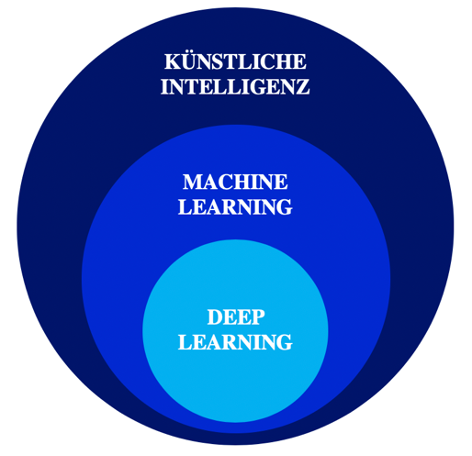
\includegraphics[scale=1.0]{content/pics/Picture_2.png}
\caption{Zusammenhang von KI, ML und Deep Learning. Eigene Erstellung in Anlehnung an \cite{Kelleher}}
\label{Abbildung:kelleher}
\end{figure}

Das Ziel der künstlichen Intelligenz ist es Systeme aufzubauen, die Aufgaben lösen können, die Intelligenz auf Niveau des Menschen voraussetzen. Machine Learning wird dabei als Teilmenge bzw. Teildisziplin der künstlichen Intelligenz eingeordnet \cite[S. 14]{Gupta}.

Machine Learning ermöglicht es Computern, aus Erfahrungen beziehungsweise aus Aufzeichnungen Regeln zu lernen, ohne explizit programmiert zu werden \cite{samuel}. Gängig ist im Bereich Machine Learning eine Unterscheidung zwischen drei Arten des Lernens: dem überwachten Lernen, dem unüberwachten Lernen, und dem sogenannten Reinforcement Learning. 

Beim überwachten Lernen existiert in Trainingsdaten für jedes Beispiel eine Beschriftung. Mit Hilfe der Beschriftungen (oder auch Klassen) kann nun beispielsweise ein Klassifikationsmodell gelernt werden. Das so erzeugte Modell wird anschließend genutzt, um eine Vorhersage der Klassen von neuen, unbekannten Datensätzen zu realisieren. Auch die Erstellung von Regressionsanalysen zählt zur Kategorie des überwachten Lernens. Dabei werden keine diskreten Klassen geschätzt, sondern stetige, kardinale Werte. Das unüberwachte Lernen verzichtet auf beschriftete Beispiele. Entsprechende Verfahren können etwa Cluster bilden, die ähnliche Datensätze zusammenfassen (Clustering). Auch die Ausreißererkennung, sowie das Lernen von Assoziationsregeln fallen in die Kategorie des unüberwachten Lernens. Assoziationsregeln sind etwa bei Warenkorbanalysen hilfreich, wenn häufig gemeinsam gekaufte Produkte identifiziert werden sollen. Beim Reinforcement Learning werden sogenannte Belohnungen (Rewards) und Strafen (Penalties) verwendet, um beispielsweise Bots das Spielen von Computerspielen beizubringen \cite[S. 7-15]{Geron}.

Deep Learning (DL) beschreibt eine Gruppe von Verfahren innerhalb der Domäne des maschinellen Lernens, bei der neuronale Netzwerke eingesetzt werden. Bei künstlichen neuronalen Netzen handelt es sich um eine Gruppe von Machine-Learning-Algorithmen, die inspiriert sind von natürlichen neuronalen Netzen aus der Natur \cite[S. 2]{White}. Das Wort deep in Deep Learning bezieht sich auf die Anzahl der Schichten des Netzwerks, durch das Eingaben verarbeitetet werden. Abbildung \ref{Abbildung:Nielsen} zeigt exemplarisch ein einfaches Artficial Neural Network (ANN). Deep Neural Networks (DNNs) sind stets mit mehr als einem sogenannten Hidden Layer ausgestattet. Das sind die Schichten des Netzwerks, in denen die Verarbeitung der Eingaben stattfindet \cite{Nielsen}. 

\begin{figure}[h]
\centering
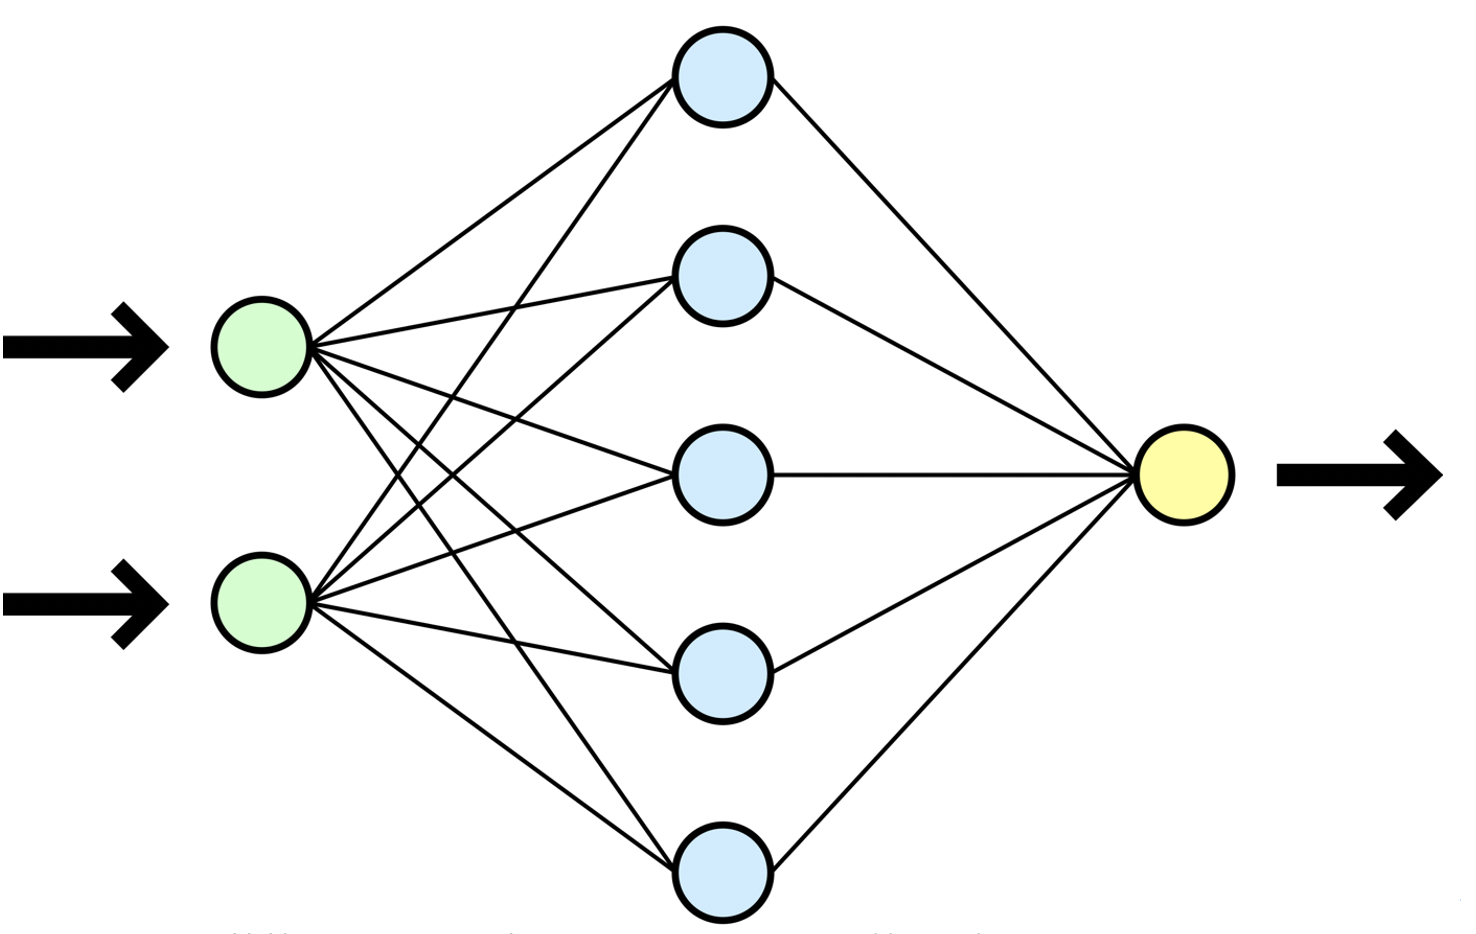
\includegraphics[scale=0.5]{content/pics/Picture_3.png}
\caption{Ein neuronales Netz mit je einem Input-, Hidden- und Output-Layer, aus \cite{Nielsen}}
\label{Abbildung:Nielsen}
\end{figure}

Es gibt neben ANNs und DNNs noch weitere Architekturansätze zur Realisierung von neuronalen Netzen. Einige davon, wie Recurrent Neural Networks (RNNs), sind für bestimmte Aufgaben besser geeignet als andere. RNNs sind insbesondere für die Verarbeitung von natürlicher Sprache von Bedeutung. Es können verschiedene Formen von RNNs unterschieden werden, wobei für den Anwendungsfall der Sprachverarbeitung insbesondere Encoder-Decoder-RNNs hervorzuheben sind, die auch als seq2seq-Modelle bezeichnet werden und besonders gut mit Sequenzen (z. B. Abfolgen von Wörtern) umgehen können. Gemeint ist hier etwa eine Übersetzung, die eine Sequenz als Eingabe benötigt und eine Übersetzung als Sequenz wieder ausgibt. \cite[23-28]{White} Convolutional Neural Networks (CNNs) sind hingegen unter anderem für den Bereich Computer Vision (Bildverarbeitung/ Bilderkennung) von großer Bedeutung. Sie wurden explizit für diese Aufgabe entwickelt \cite[]{LeCun}.

Die verschiedenen neuronalen Netze haben die Gemeinsamkeit, dass sie Neuronen (Knoten) und gewichtete Verbindungen (Kanten) zwischen den Neuronen beinhalten. Neuronen werden aktiviert durch Eingaben und verarbeiten diese mit bestimmten Funktionen weiter, um wiederum eine Ausgabe zu generieren. Das Ermitteln der Gewichtungen dieser Verbindungen wird als Training bezeichnet. Das Training des Netzes besteht aus dem Lösen eines hoch-dimensionalen, nichtlinearen, nicht-konvexen und globalen Optimierungsproblems. Es kann erfolgen unter Zuhilfenahme der Algorithmen Gradient Descent und Backpropagation \cite[1-13]{White}.

Während bei herkömmlichen Machine-Learning-Ansätzen Features (auch: Attribute oder Eigenschaften von Datensätzen), die während der Verarbeitung benötigt werden, manuell von Menschen gebildet werden müssen, werden diese Features bei Deep-Learning-Ansätzen durch das neuronale Netz erzeugt \cite[S. 3-4]{Alom}. Durch diesen Vorteil sind bessere Ergebnisse möglich \cite[S. 11]{Alom}. 

\section{Natural Language Processing}

Es geht nachfolgend um Techniken zur Verarbeitung und Auswertung von Texten und natürlicher Sprache (Engl.: Natural Language Processing, Abk.: NLP).  NLP kann dabei als Teil des umfangreichen Gebiets Text Mining verstanden werden \cite[S. 17]{Perez}. Das Verständnis von natürlicher Sprache (Engl.: Natural Language Understanding, Abk.: NLU) gilt als Voraussetzung für die Schaffung eines vollständigen KI-Systems, wodurch der Bezug von Sprachverständnis bzw. der Sprachverarbeitung zur KI gegeben ist \cite[S. 8]{Yampolskiy}.

\subsection{Vorverarbeitung von Texten}

Eine geeignete Vorverarbeitung (Engl.: Preprocessing) von Texten gilt als Voraussetzung für den Erfolg der späteren Auswertungen \cite[S. 46]{Anandarajan}. Daher werden hier zunächst einige der gängigen Schritte zur Vorverarbeitung von Texten skizziert und grundlegende Methoden erläutert.

Bei der Token-Erstellung (Engl.: Tokenization) wird Text in sogenannte Tokens unterteilt. Im einfachsten Fall bestehen Tokens aus einem Wort – dann handelt es sich um Unigramme (Engl.: unigram). N-Gramme (Engl.: n-grams) stellen eine Alternative zu Unigrammen dar. N-Gramme sind Wort-Sequenzen mit der Länge n \cite[S. 48]{Anandarajan}. Stoppworte dienen zwar einem grammatikalischen Zweck, in Bezug auf den Inhalt von Texten erbringen sie aber nur einen geringen Mehrwert. Aus diesem Grund werden Stoppworte im Rahmen der Vorverarbeitung in der Regel aus Texten entfernt. Dazu kann z. B. ein Wörterbuch verwendet werden, das bekannte Stoppworte wie z. B. [und, er, ein, hat, …] enthält \cite[S. 50-53]{Anandarajan}. Die Reduktion von Begriffen auf die Stammform (Engl.: Stemming) verfolgt das Ziel, verschiedene grammatische Varianten des gleichen Wortes zu vereinheitlichen, um die Gesamtanzahl der unterschiedlichen Wörter innerhalb eines Textkörpers zu reduzieren. Die Erzeugung der Stammformen erfolgt z. B. durch den Porter-Stemmer, der Stammformen auf Basis von Regeln bilden kann. Die Lemmatisierung (Engl.: Lemmatization) führt Begriffe auf eine Art ``Wörterbuchform`` zurück und kann dadurch besser interpretierbare Ergebnisse liefern als das Stemming \cite[S. 30-32]{Manning} Worttypen wie Adjektive, Verben, Substantive, etc. werden erkannt und markiert durch Part-of-Speech-Tags (Abk.: POS-Tags). Zur Realisierung dieser Markierung können Text-Korpora verwendet werden, bei denen manuell Wörter mit den entsprechenden Wortarten markiert wurden \cite[S. 58]{Anandarajan}.

\subsection{Repräsentation von Texten} 

Nach den beschriebenen Schritten zur Vorverarbeitung von Textdokumenten kann die Darstellung von Begriffen im Verhältnis zu Dokumenten über eine Term-Document-Matrix (TDM) erfolgen (vgl. Tabelle \ref{tab:tdm}). Die transponierte Variante dieser Matrix heißt Document-Term-Matrix (DTM) \cite[S. 61ff]{Anandarajan}. Eine TDM könnte so etwa nach der initialen Vorverarbeitung aussehen.

\begin{table}[h]
\centering
\begin{tabular}{|c|c|c|c|c|}
\hline
\textbf{}     & \textbf{Dokument\_1} & \textbf{Dokument\_2} & \textbf{Dokument\_3} & \textbf{...} \\ \hline
\textbf{dog}  & 0                    & 0                    & 2                    & ...          \\ \hline
\textbf{cat}  & 1                    & 1                    & 0                    & ...          \\ \hline
\textbf{bird} & 3                    & 0                    & 1                    & ...          \\ \hline
...           & ...                  & ...                  & ...                  & ...          \\ \hline
\end{tabular}
\caption{Beispiel für eine TDM. Fiktives Beispiel in Anlehnung an \cite[S. 62]{Anandarajan}}
\label{tab:tdm}
\end{table}

In dieser Art der Darstellung wird die Menge der Wörter eines Dokuments als Bag-of-Words bezeichnet \cite[S. 46]{Anandarajan}. Die Ausprägungen in den Zellen der Tabelle \ref{tab:tdm} beschreiben in diesem Beispiel die Häufigkeit des Vorkommens der Begriffe in den jeweiligen Dokumenten. Um zur Term Frequency (Abk.: tf) zu gelangen, ist die Anzahl des Begriffs durch die Gesamtanzahl der Begriffe im jeweiligen Dokument zu dividieren. Für den Begriff cat ergibt sich für Dokument\_1 (erste Spalte) eine tf von \( \frac{1}{4} \), unter Vernachlässigung der Spalten und Zeilen ohne kardinale Ausprägungen (Spalten mit Ausprägung ...).

Eine weitere, für die spätere Auswertung relevante Kennzahl heißt Document Frequency (Abk. df). Dabei wird zunächst die Häufigkeit der Begriffe reduziert auf eine binäre Angabe 1 oder 0, die Häufigkeit wird also vernachlässigt und es verbleibt lediglich eine Information darüber, ob ein Wort in den Dokumenten vorkommt oder nicht. Die nun erzeugten Werte werden zeilenweise addiert, um die Kennzahl df zu erhalten. Das Beispiel ``cat`` aus Tabelle \ref{tab:tdm} würde zu einer df von 1+1+0=2 führen. Der Wert df gibt damit an, in wie vielen Dokumenten ein Begriff vorkommt. Um seltenen, und damit aussagekräftigen Begriffen ein höheres Gewicht zu geben als Begriffen, die zwar häufig vorkommen, dafür aber auch weniger Relevanz und Wirkung haben, existiert mit der inversen Dokumenten-Häufigkeit (Engl.: inverse document frequency, Abk.: idf) eine weitere Metrik. Sie wird berechnet als:

\[ idf_i = \log_2( \frac{n}{df_i}) + 1 \]

wobei n die Anzahl der Dokumente ist, und df wie oben beschrieben berechnet wird. Die hier beschriebenen Metriken können kombiniert werden zur tf-idf-Metrik. Dabei wird tf mit idf lediglich multipliziert. Für den Beispielbegriff cat ergibt sich unter Vernachlässigung der Spalten und Zeilen ohne kardinale Ausprägungen ein Wert von \( \frac{1}{4} \times ( \log_2( \frac{3}{2} )+1)=0,39 \) 
für das erste Dokument. Der tf-idf-Wert von Begriffen kann nun als Ausprägung in den Zellen einer TDM an Stelle der schlichten Anzahl der Begriffe verwendet werden \cite[S. 61-73]{Anandarajan}.

Die tf-idf-Metrik ist bei der Betrachtung von mehreren Begriffen zusammengefasst eine Grundlage für die Erkennung von wichtigen Begriffen. Dabei sollten die Dokumente möglichst einen Bezug zueinander haben. Ein Beispiel wäre eine Menge von Dokumenten über Software-Entwicklungsprojekte. In jenen Dokumenten würde der Begriff ``Software`` häufig vorkommen. Die Bedeutung des Begriffs ist allerdings eher gering, da er wahrscheinlich in allen Dokumenten vorhanden sein wird. Beim tf-idf-Maß erhalten seltene Begriffe einen hohen Wert, wodurch solche Begriffe als interessant identifiziert werden können. \cite[S. 107-110]{Manning}. Auf Basis der einfachen TDM oder auch auf Basis der erweiterten Variante unter Verwendung von tf-idf-Werten können im Anschluss Verfahren des maschinellen Lernens verwendet werden, wie im praktischen Teil der Arbeit gezeigt wird.  

\subsection{Regelbasierte Ansätze}

Um ein ML-Modell trainieren zu können, sind Trainingsdaten notwendig (vgl. Kapitel 2.1). Wenn diese nicht in ausreichender Menge vorhanden sind, dann kann ein regelbasierter Ansatz eine Alternative zu Verfahren des maschinellen Lernens sein. Regelbasierte Systeme zählen zu den ältesten Ansätzen im Bereich NLP und haben sich in der Praxis bewährt. Aus technischer Sicht können für die Realisierung eines regelbasierten Ansatzes etwa String-Vergleiche (z. B. mit regulären Ausdrücken zur Entdeckung bestimmter Muster) verwendet werden. Auch mit kontextfreien Grammatiken können Regeln ausgedrückt werden \cite{kaggle}. Ein simpler endlicher Automat kann verwendet werden, um einfache Regeln zu beschreiben \cite[S. 219]{Manning}. Zu den regelbasierten Ansätzen werden hier explizit auch Wenn-Dann-Regeln gezählt \cite[S. 23ff.]{Ertel}. Beispiele für Entitäten, die gut über einen regelbasierten Ansatz erkannt werden können, sind etwa IP-Adressen, URLs, oder Telefonnummern \cite{spacy}.

Über Ontologien oder Taxonomien können ebenfalls Entitäten erkannt werden. Solche Wissensbasen galten früher als grundlegender Baustein von KI-Systemen. Ein solcher Bestand kann zu Beginn eines Projekts erstellt werden und dann im Laufe der Zeit weiterentwickelt werden. Ontologien führen in diesem Kontext zu wiederverwendbaren, erweiterbaren Wissensbeständen. Sie können sowohl von Menschen als auch von Computern verstanden werden und bilden Mengen von explizit definierten Terminologien ab. Die grundlegenden Begriffe, also das Vokabular einer bestimmten Domäne und die Beziehungen der Begriffe untereinander werden in einer Ontologie modelliert \cite[S. 37-55]{ontologies}. Das Vokabular könnte in den erwähnten Wenn-Dann-Regeln verwendet werden. Die Begriffe Ontologie und Topic werden in der Literatur und daher auch hier als Synonyme verwendet. 

Taxonomien können ebenfalls für solche Klassifizierungszwecke verwendet werden. Eine Taxonomie hat einen Namen und besteht aus Beispielen. Es kann flache bzw. einfache Taxonomien geben, aber auch hierarchische, oder gar vernetzte Taxonomien \cite{inmon}

Da im Titel dieser Arbeit die Evaluation von ausgewählten ML-Verfahren festgelegt ist, werden regelbasierte Ansätze im praktischen Teil der Arbeit weniger ausführlich betrachtet als ``echte`` ML-Ansätze. Sie gelten aber in realen Szenarien als mögliche Option für bestimmte Anwendungsfälle und wurden daher hier beschrieben.

\subsection{Vektorbasierte Ansätze}

Die Begriffe Wort-Vektor und Wort-Einbettung (Engl.: Word Embedding) werden hier als Synonyme verwendet, wie in \cite[S. 38]{White}. Als moderner Algorithmus zur Erzeugung von Wort- Einbettungen gilt Word2Vec. Entwickelt wurde das Verfahren von Google-Forschern \cite{mikolov2013}, allerdings sind auch andere Unternehmen an der Weiterentwicklung dieser Ansätze beteiligt. So gibt es etwa mit fastText von Facebook oder mit GloVe der Stanford University ebenfalls Möglichkeiten zur Nutzung von vorbereiteten Word-Vektoren sowie für das Training eigener Wort-Vektoren \cite{facebook} \cite{stanford}. Word2Vec versucht, die Probleme des Bag-of-Word-Ansatzes beziehungsweise der One-Hot-Encodings zu vermeiden. Durch diese Repräsentation – bei der das Vorhandensein eines Wortes in einem Textdokument etwa mit einer 1 angezeigt wird und das Fehlen mit einer 0 – entstehen hoch-dimensionale Tabellen mit vielen Zeilen. Dabei kommt häufig der Wert 0 als Ausprägung vor. Damit einher geht ein gewisser Informationsverlust, da Kontextinformationen (z. B. die Position der Wörter innerhalb der Dokumente) verloren gehen  und weil viele ML-Verfahren mit Daten, die in dieser Art und Weise repräsentiert sind, schlecht umgehen können. Zu viele Spalten können zu einem zu zu komplexen Modell führen, was nicht erwünscht ist. \cite[S. 145]{knime}. Als Architektur für das Erzeugen von Wort-Vektoren kommt bei Word2Vec ein voll-verknüpftes neuronales Feed-Forward-Netz zum Einsatz. Eine Eigenschaft des Verfahrens ist, dass bei jedem Wort der Kontext des Worts in gewissem Maße erhalten bleibt. Die Anwendung von Word2Vec führt zu den sogenannten Einbettungen, was letztendlich einer deutlich kompakteren Darstellung der Informationen entspricht, als das etwa bei der Darstellung von Text in Form einer Term-Document-Matrix der Fall ist. Eine Einbettung entspricht einer Darstellung von Begriffen in Vektorform. Die mit Word2Vec erzeugten Wort-Vektoren können als Eingabe für weitere Machine-Learning-Verfahren verwendet werden, wobei diese Repräsentation deutlich bessere Resultate etwa bei Klassifizierungsaufgaben verspricht, als in der unverarbeiteten Form. Um die Vektoren zu erzeugen, wird ein neuronales Netz trainiert, welches das Ziel hat, die Wahrscheinlichkeit von bestimmten Kontextwörtern einzelner Wörter vorherzusagen (im sogenannten Skip-Gram-Ansatz). Die internen Gewichtungen des neuronalen Netzes werden letztendlich als Wort-Vektoren verwendet. \cite[S. 148-160]{knime}. 

Neben Wort-Einbettungen kommen an dieser Stelle noch Dokumenten-Einbettungen in Betracht. Der Algorithmus dazu heißt Paragraph Vector. Im Vergleich zu Word2Vec werden für das Erstellen der Einbettungen zusätzlich zu den Wörtern auch jeweils Paragraphen in das Training der Vektoren mit einbezogen. Die Paragraphen liefern also zusätzlichen Kontext. Vergleichbar ist der Paragraph mit einer Angabe darüber, wo im Dokument bzw. auch in welchem Dokument sich ein Begriff in den Trainingsdaten befunden hat \cite{mikolov2014}. Eine Implementierung von Dokument-Einbetttungen findet sich unter dem Namen doc2vec \cite{rehurek}.

In Abbildung \ref{Abbildung:mikolov} dargestellt sind einzelne Wörter, die als Vektoren abgebildet werden. Die Abkürzung W steht aus mathematischer Sicht für eine Matrix, die einzelnen Wort-Vektoren sind als Spalten in dieser Matrix enthalten. Nach Bildung der initialen Vektoren werden diese konkateniert (``aufsummiert``), um den sogenannten Kontext abzubilden. In diesem Beispiel wird ein neuronales Netz verwendet, das die Wahrscheinlichkeit des Wortes ``on`` im Kontext der Begriffe ``the cat sat`` ermittelt. Hier dargestellt ist das Continuous Bag of Word-Modell (CBOW), das genaue Gegenteil von Skip-Gram, das oben bereits erwähnt wurde. Bei der Verwendung des Paragraph-Vector-Ansatzes wird jeder Paragraph als Spalte in einer Matrix D abgebildet. Diese zusätzliche Information ergänzt den beschriebenen Kontext. Was genau als Paragraph definiert wird, kann frei gewählt werden. Es kann sich um längere Abschnitte, ganze Dokumente, oder auch eine Auswahl von Sätzen handeln \cite{mikolov2014}.
 
\begin{figure}[h]
\centering
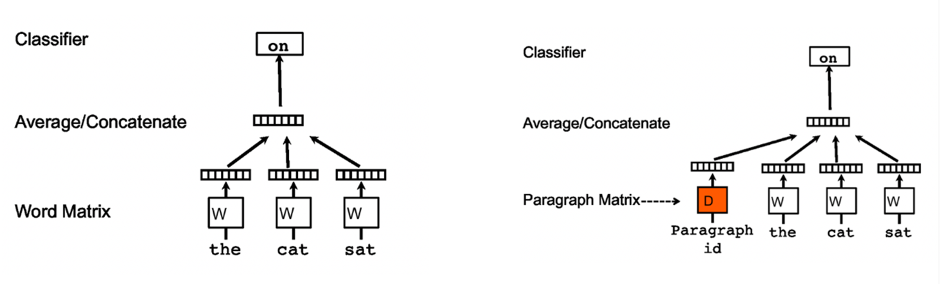
\includegraphics[scale=0.9]{content/pics/Picture_5.png}
\caption{Funktionsweise von Word2Vec (links) und von Paragraph Vector (rechts), aus \cite{mikolov2014}}
\label{Abbildung:mikolov}
\end{figure}

Einbettungen müssen nicht für jede Anwendung neu trainiert werden. Stattdessen können auch vor-trainierte (pre-trained) Einbettungen wiederverwendet werden, wie am Anfang dieses Abschnitts bereits angedeutet wurde. Unten dargestellt (Abbildung \ref{Abbildung:word_vecs}) ist ein Ausschnitt aus dem bereits trainierten GloVe-Modell, der die Vektor-Repräsentation verdeutlichen soll. Es wurde trainiert auf Basis des Korpus Wikipedia 2014 \cite{stanford}. Die Abbildung soll verdeutlichen, dass mit den Vektoren eine mathematische Repräsentation von Begriffen gefunden wurde. Die Wörter können damit für verschiedene Rechenoperationen verwendet werden. Einige davon werden im praktischen Teil dieser Arbeit erprobt. 

\begin{figure}[h]
\centering
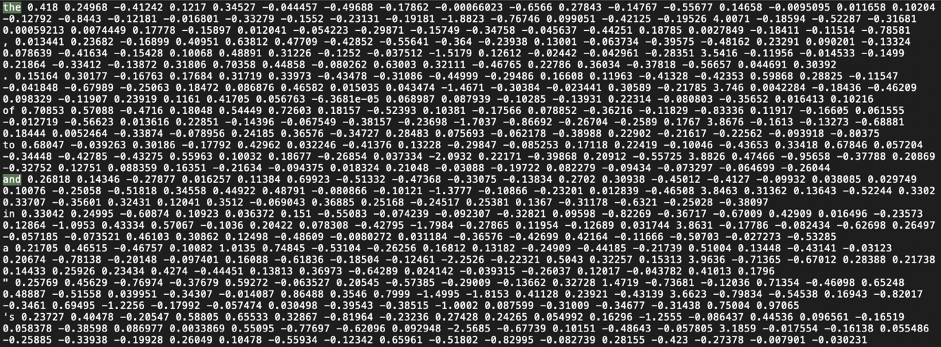
\includegraphics[scale=0.9]{content/pics/Picture_6.png}
\caption{Vektoren der Begriffe ``the`` \& ``and``. Eigene Bildschirmaufnahme.}
\label{Abbildung:word_vecs}
\end{figure}
 
Die größeren NLP-Modelle, etwa von spaCy, beinhalten standardmäßig nutzbare Wortvektoren. Eine eigene Untersuchung ergibt, dass diese Modelle auch gewisse fachspezifische Wörter berücksichtigen, etwa die Begriffe Shipments oder containerization. Allerdings existieren für reale Begriffe wie Projekt- oder Systemnamen aus einem spezifischen Unternehmen keine Wortvektoren. Solche Begriffe nennt man out-of-vocabulary \cite{spacy2}. Das erschwert die Verwendung von Modellen, die ``gebrauchsfertig`` zur Verfügung stehen. 

\subsection{Transformer-Ansätze}
Transformer werden erstmals Ende 2017 eingeführt. Laut den Autoren der Erstveröffentlichung ist der Ansatz in der Lage, bessere Ergebnisse in bestimmten Bereichen zu erzielen als bisherige Ansätze auf Basis von RNNs oder CNNs; zudem ist das Training parallelisierbar und damit schneller als bei früheren Ansätzen \cite{Vaswani}. Transformer-Ansätze können für viele NLP-Teilbereiche verwendet werden, etwa für Named-Entity-Recognition, Übersetzungen, das Generieren von Zusammenfassungen, und weitere Anwendungsfälle. \cite[S. 25-26]{Gupta}. Die Nutzung von vortrainierten Modellen wird als Transfer-Learning bezeichnet. Transformer können dies ermöglichen. Gewisse Gewichtungen innerhalb von neuronalen Netzen können dabei übernommen werden und müssen nicht neu trainiert werden (z. B. grundlegende Sprach-Eigenschaften). Vortrainierte Modelle sind eine Option, wenn nur wenige Daten für das Training zur Verfügung stehen. Die vor-trainierten Modell erfahren eine Fein-Abstimmung (Engl.: Fine-Tuning), wodurch die Modelle an den jeweiligen Anwendungsfall angepasst werden \cite[S. 45-56]{Alom}.
Ein konkreter Transformer-Ansatz ist BERT (Bidirectional Encoder Representations from Transformers). Es gibt eine Pre-Training-Phase und eine Fine-Tuning-Phase, durch die das finale Modell erzeugt wird. Es wurden Ergebnisse in diversen NLP-Referenzproblemen (Beispiel: Beantwortung von Fragen) erreicht, die als state-of-the-art bezeichnet werden können \cite{devlin}. 
GPT (Generative Pre-trained Transformer) und seine Nachfolger GPT-2 und GPT-3 sind weitere Beispiele für Transformer-Modelle, die insbesondere für die Text-Erzeugung eingesetzt werden können \cite{Brown}

\section{Das Application-Portfolio-Management als Teil der IT-Governance}

IT-Governance soll sicherstellen, dass Informationstechnologie (IT) die Strategien und Ziele von Unternehmen unterstützt. Die IT soll so angepasst und weiterentwickelt werden, dass relevante Anforderungen erfüllt werden. Dazu zählen insbesondere regulatorische und gesetzliche Anforderungen \cite[S. 5]{reiss}. Gemeint sind damit etwa Gesetze und Rechtsverordnungen, wie die Datenschutzgrundverordnung (DSGVO), der Sarbanes-Oxley-Act (SOA), oder auch die bankaufsichtlichen Anforderungen an die IT (BAIT) im Bankenumfeld \cite[S. 274-275]{gaulke}. 

Außerdem kann davon ausgegangen werden, dass Manager stets auch weitere, individuelle Interessen aus ihrem Arbeitskontext im Sinn haben, wenn die Notwendigkeit von IT-Governance begründet werden soll. Risiken, die mit dem Betrieb von IT-Systemen einhergehen, sollten dem Management bekannt sein, damit entsprechende Maßnahmen getroffen werden können. Außerdem ist von Interesse, welchen fachlichen Mehrwert einzelne Systeme tatsächlich bringen und welche Geschäftsbereiche durch die Systeme unterstützt werden. Der große Vorteil von IT-Governance ist erhöhte Transparenz. Die Transparenz macht unter anderem Kosten sichtbar und ermöglicht sinnvolle Entscheidungen im Zusammenhang mit der Unternehmens-IT  \cite[S. 5-7]{ncc}. Mit den angesprochenen Risiken können (u. a.) wirtschaftliche Verluste im Falle von Systemausfällen verbunden sein, aber auch der langfristige Verlust der eigenen Wettbewerbsfähigkeit, wenn zu lange mit der Erneuerung von Systemen gewartet wird  \cite[S. 20]{ncc}. IT-Governance ist ein Bestandteil eines übergeordneten Corporate-Governance-Ansatzes, bei dem es um die Steuerung und Überwachung eines gesamten Unternehmens geht \cite[S. 2]{gaulke}. 

\subsection{COBIT als mögliche Grundlage für das APM?}

Das Rahmenwerk (Engl.: Framework) COBIT kann als methodische Grundlage für IT-Governance dienen. Die Abkürzung steht für Control Objectives for Information and Related Technology. Die aktuelle Version (während der Bearbeitungszeit dieser Arbeit) ist COBIT 2019 \cite[S. 9-12]{gaulke}. 

COBIT definiert in seinem Kern-Modell (vgl. Abbildung \ref{Abbildung:isaca}) sogenannte Governance- und Management-Ziele \cite[S. 67]{gaulke}. Ziel APO05 heißt ``Managed Portfolio``. Anhand dieses Beispiels soll verdeutlicht werden, dass der Umgang mit bestimmten Portfolios ein wesentlicher Bestandteil von Governance-Tätigkeiten sein kann. Die Bezeichnung Application-Portfolio wird hier allerdings nicht verwendet, sondern es geht stattdessen um Projekte und Programme. Dabei müssen einzelne Projekte oder Programme priorisiert werden, damit strategische Ziele erreicht werden können \cite[S. 87-92]{isaca1}. 

Statt einem eigenen Management-Ziel zum Umgang mit Applikationen exisitert in COBIT die Empfehlung zu ``Managed Assets`` (``Betriebsmitteln``, vgl. Ziel BAI09) \cite[S. 209-214]{isaca1}, wozu auch der Umgang mit Software-Lizenzen zählt. Unter dem Ziel ``Managed Configuration`` (BAI10) wird empfohlen, Daten zu ``wichtigen Ressourcen`` zu erheben und zu verwalten \cite[S. 73]{gaulke}. Unter Ziel APO03 wird das Managen der Unternehmensarchitektur empfohlen, was die Einrichtung einer Referenzarchitektur beinhaltet, in der u. a. auch Anwendungen und Technologien berücksichtigt werden können \cite[S. 70]{gaulke}. In welchen Variationen diese Empfehlungen in Unternehmen ganz konkret umgesetzt werden, ist diesen stets selbst überlassen \cite[S. 65]{gaulke}.
 
\begin{figure}[h]
\centering
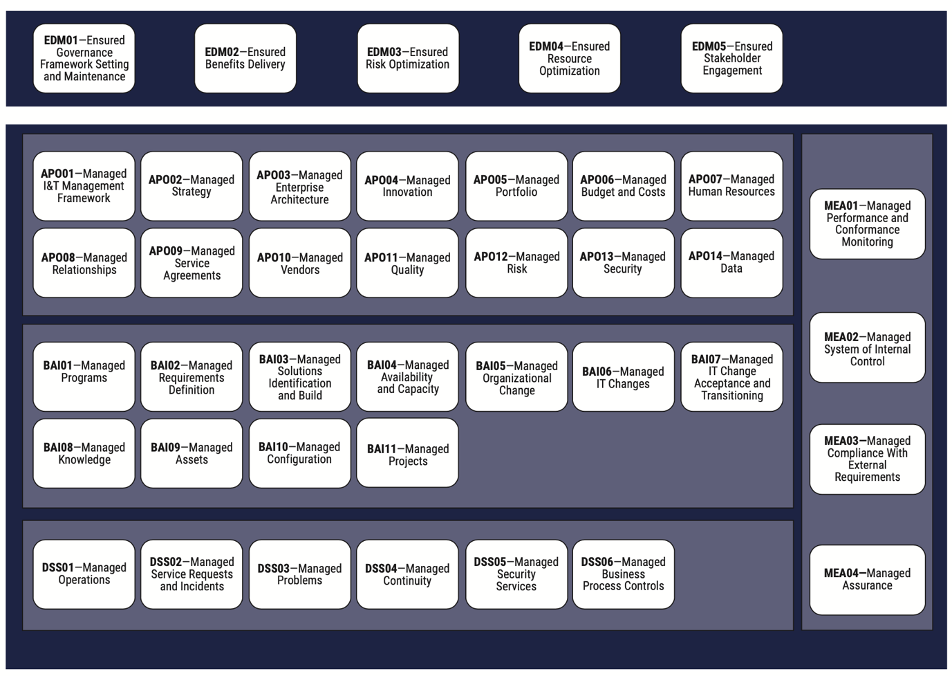
\includegraphics[scale=0.9]{content/pics/Picture_7.png}
\caption{COBIT-Kernmodell, aus \cite[S. 21]{isaca2}}
\label{Abbildung:isaca}
\end{figure}

Neben COBIT gibt es weitere Frameworks, bzw. Modelle zum Umgang mit einzelnen Governance-Themen. In \cite[S. 127-133]{gaulke} werden beispielsweise das CMMI - Capability Maturity Model (Integration) sowie die IT Infrastructure Library (ITIL) erwähnt. 
 
Außerdem gibt es spezielle (Enterprise-)Architektur-Frameworks. Auf einige davon wird in einem späteren Abschnitt kurz eingegangen. 

\subsection{Die Rolle von Textdokumenten für die IT-Governance}
Verschiedene IT-Projekte eines Unternehmens und damit verbunden auch Softwareentwicklungsprojekte stehen grundsätzlich in Konkurrenz zueinander. Mehrere Stakeholder möchten, dass ihr eigenes Projekt mit Priorität behandelt wird und erfolgreich umgesetzt wird. Dazu kommt, dass es Abhängigkeiten zwischen den einzelnen Vorhaben geben kann (Beispiel: Der Abschluss von Projekt A ist eine Voraussetzung für die erfolgreiche Umsetzung von Projekt B). Aus diesem Grund ist es wichtig, dass das IT-Management die Gesamtheit der Projekte im Blick hat, und sich weniger nur auf einzelne Projekte fokussiert \cite[S. 1]{frey}. Ein Portfolio muss also verwaltet und gesteuert werden.

Neben dem voraussichtlichen Return on Investment (ROI) der sich durch die Umsetzung eines Projekts ergibt, müssen weitere Faktoren vor der Umsetzung von Projekten geschätzt werden. Dazu zählt das Risiko, das mit einem Projekt einhergeht \cite[S. 120ff.]{gadatsch}. Zunächst können für diese Schätzung die bereits erstellten Dokumentationen in Betracht gezogen werden. Der Begriff der Dokumentation bezeichnet in der Regel nachträglich erstellte Beschreibungen von Projekten. Unter dem Begriff können allerdings auch die zu einem noch laufenden oder geplanten Projekt gehörenden Dokumente verstanden werden. Dokumentationen erfüllen neben der Aufzeichnung von Ideen in Software-Entwicklungs-Projekten einen weiteren wichtigen Zweck: Sie gelten als wesentliches Werkzeug zur Umsetzung von Governance und zur Sicherstellung von Compliance \cite[S. 2]{reiss}. Diesen Zweck erfüllen sie, wenn Außenstehende die bereits abgeschlossenen oder geplanten Projekte oder Anwendungen bewerten müssen, um letztendlich Entscheidungen zum Umgang mit diesen treffen zu können. Deshalb wird in dieser Arbeit angenommen, dass Dokumentationen in Text-Form von hoher Bedeutung für die Gestaltung der Projekt- und Applikationslandschaft von Unternehmen sind. Die Güte von Dokumentationen ist dabei von entscheidender Bedeutung. Ein Dokumentationsmanagementsystem kann bei der Erstellung von anforderungsgerechten Dokumenten unterstützen. Dabei können verschiedene Vorgaben an die Struktur der Dokumente gemacht werden \cite[S. 29]{reiss}. Dazu zählt beispielsweise eine bestimmte Kapitelstruktur. Diese kann von einer Einteilung der Dokumente zu bestimmten Dokumententypen abhängig gemacht werden \cite[S. 34-39]{reiss}.

\subsection {Das APM und verwandte Begriffe}
Es gibt im Zusammenhang mit der Idee des Application-Portfolio-Management in der Literatur diverse ähnliche Begriffe, die im Kern das beschreiben, was in dieser Arbeit unter APM verstanden wird. Ein solcher Begriff aus einer frühen Veröffentlichung zu APM ist etwa das IT Portfolio Management. Hier wird von stetigen ``Kaufs-, Verkaufs- und Beibehaltungs-Entscheidungen`` gesprochen, um sogenannte IT-Portfolios zu gestalten bzw. um sie stets zu optimieren. APM bildet laut den Autoren gemeinsam mit dem Project Portfolio Management sowie dem IT Asset und Infrastructure Management die Disziplin des IT Portfolio Managements \cite[S. 2-14]{Gliedman}.

Das oben bereits erwähnte Enterprise Architecture Management (EAM) verfolgt einen umfangreicheren, ganzheitlichen Ansatz zur Darstellung, Gestaltung und Weiterentwicklung der gesamten Systemlandschaft von Unternehmen. Es werden sowohl die Prozess- als auch die Systemwelt strukturiert betrachtet. Dabei geht es stets auch um die Schaffung von Transparenz. Durch eine solche Transparenz können etwa unnötig redundante Systeme erkannt bzw. vermieden werden \cite[S. 7-10]{Bitkom}. Mit unnötig redundanten Systemen sind solche Systeme gemeint, welche Geschäftsfunktionen abdecken, die bereits durch andere Systeme oder Anwendungen unterstützt werden. Eine Business Support Matrix kann solche Beziehungen zwischen Anwendungen und Geschäftsfunktionen (auch: Capabilities) visualisieren \cite{jung1}. 
Der Umfang von EAM wird dargestellt in Abbildung \ref{Abbildung:ea}. Die Abbildung soll verdeutlichen, dass der Fokus nicht wie im APM nur auf Applikationen (hier repräsentiert am ehesten durch den Kasten Anwendungsarchitektur) liegt, sondern dass sich EAM mit weiteren Ebenen beschäftigt (etwa mit der Geschäftsarchitektur oder auch mit der Strategie).
 
\begin{figure}[h]
\centering
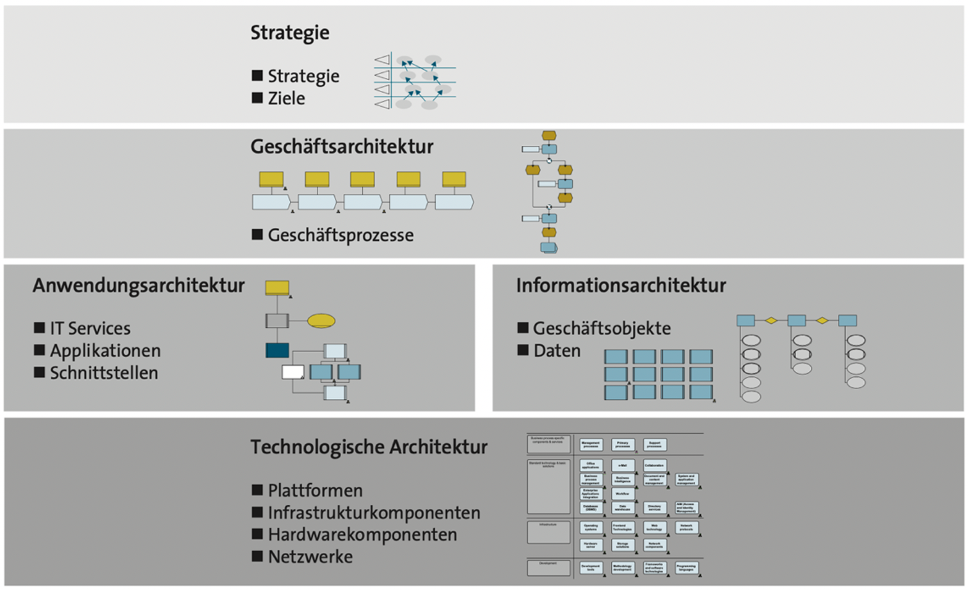
\includegraphics[scale=0.9]{content/pics/Picture_8.png}
\caption{EA-Überblick, aus \cite[S. 13]{Bitkom}}
\label{Abbildung:ea}
\end{figure}

Der enge Bezug von APM und EAM zeigt sich außerdem in Rahmenwerken, wie dem Architekturframework der Open Group (TOGAF). Dort zählt z. B. der Application Portfolio Catalog zu den grundlegenden Artefakten, die bei der Gestaltung einer Architektur nach TOGAF zu berücksichtigen sind. Schnittstellen zwischen Applikationen werden in dem Framework in einem Interface Catalog dokumentiert. Damit sind u. a. Abhängigkeiten visualisierbar und zentrale Anwendungen identifizierbar \cite[Kap. 31]{togaf}. Im Department of Defense Architecture Framework (DoDAF) gibt es verschiedene sogenannte Viewpoints, die wiederum aus mehreren Views bestehen können. Ein Viewpoint in diesem Framework ist die Systems-Viewpoint. Eine konkrete View ist z. B. die ``System Interface Description`` (SV-1). In ihr werden alle Systeme, die von Interesse sind, inklusive Schnittstellen zu anderen Systemen dargestellt. Die View ist vergleichbar mit dem TOGAF Interface Catalog. Es kann in anderen Views auch z. B. um die Unterstützung ``operationaler Aktivitäten`` durch Software-/ oder System-Funktionen gehen (SV-5). Ein Beispiel wäre die Dokumentation darüber, dass der operationale Prozess ``Einchecken von Passagieren``, durch ein System mit der Bezeichnung ``Airline Reservation and Ticketing System`` abgewickelt wird \cite[S. 311-344]{Rao}.

Darüber hinaus zeigt eine Befragung von Enterprise-Architekten, dass diese sich in ihrer täglichen Arbeit mit Fragen zum Umgang mit Anwendungslandschaften beschäftigen \cite{jung2}. Dazu zählen zum Beispiel Fragen wie 

\begin{itemize}
  \item Welche Anwendungen sind in Verwendung? 
  \item Welchen Zweck erfüllen einzelne Anwendungen?
  \item Welche Anwendungen sollen eingeführt oder abgeschaltet werden?
  \item Welche Redundanzen in der Anwendungslandschaft gibt es?
  \item Welche Abhängigkeiten oder Schnittstellen gibt es zwischen Anwendungen?
  \item In welchen Anwendungen werden kritische oder schützenswerte Daten gehalten?
\end{itemize}

Als Kernelement von IT-Strategien wird der IT-Bebauungsplan in einer Veröffentlichung zum Thema IT-Controlling bezeichnet. Er gibt Aufschluss über die Informationssysteme, die derzeit in einem Unternehmen im Einsatz sind. Dazu zählen (u. a.) Informationen zu Release-Ständen, zu Schnittstellen der Systeme untereinander sowie zu Geschäftsprozessen, die die von den Systemen unterstützt werden. \cite[S. 36]{gadatsch} Die Autoren dieses Beitrags nennen das IT-Portfoliomanagement als Werkzeug für IT-Controller (die dem Chief Information Officer gleichgestellt oder dieser Position direkt unterstellt sein können). Zu deren Aufgaben können die Auswahl und Steuerung von neuen Projekten oder von Wartungsprojekten gehören. \cite[S. 41-45]{gadatsch}

\subsection {Handlungsfelder des APM}
Ein grundlegendes Ziel von APM ist die Reduzierung der Komplexität von Anwendungslandschaften. Die fachlichen Anforderungen sollen bestmöglich unterstützt werden durch Anwendungen. Die Gesamtheit der Anwendungen soll jedoch eine möglichst geringe Komplexität aufweisen. Anwendungen werden dabei aus technischer (etwa Aktualität der Software), fachlicher (z. B. Eignung der Software zur Unterstützung der geschäftlichen Anforderungen) und betriebswirtschaftlicher Sicht (Betriebs- oder Lizenzkosten) untersucht. Es handelt sich um einen kontinuierlichen, andauernden Vorgang \cite{schoder}. Nachfolgend aufgelistet sind Beispiele für Fragestellungen, mit denen sich das APM befasst. Sie werden im Folgenden als Handlungsfelder des Application-Portfolio-Management zusammengefasst. Die Fragen wurden abgeleitet aus \cite{apm}. Hervorgehoben sind vier Fragen, auf die im weiteren Verlauf der Arbeit noch stärker eingegangen werden soll. Es gibt auch jeweils einen Verweis auf das jeweilige Kapitel, in denen entsprechende Verfahren zum Umgang mit den Fragen diskutiert werden.

\begin{itemize}
\item Werden bei der Implementierung von neuer Software Legacy-Systeme als Grundlage verwendet?
\item Werden die Anforderungen aus dem operativen Geschäft durch neue Anwendungen abgedeckt?
\item Sind Anwendungen aus technischer und fachlicher Sicht ``fit`` für die Zukunft?
\item Werden durch Anwendungen bestimmte rechtliche Anforderungen umgesetzt?
\item {\bf Was ist für einzelne Anwendungen ``in-scope`` und was ist ``out-of-scope``? (vgl. Abschnitt 4.3)}
\item Gibt es in den Dokumentationen der geplanten Softwareprojekte einen Projektplan oder ein Gantt-Diagramm?
\item {\bf Wurde schon einmal versucht, ein bestimmtes Vorhaben umzusetzen und wie war das Resultat? (vgl. Abschnitt 4.1)}
\item Was sind die fachlichen Anforderungen, die durch ein bestimmtes Projektvorhaben abgedeckt werden sollen?
\item Wie verhalten sich die Kosten, die durch das Ersetzen einer Software anfallen im Vergleich zu den Kosten, die bei einer Modernisierung/ Weiterentwicklung entstehen?
\item Ist es möglich, einzelne Anwendung zu verbessern/ weiterzuentwickeln?
\item Was spricht für eine Wartung einer bestehenden Software, was für eine Neuentwicklung?
\item Welche Anwendungen sind Kandidaten für eine Restrukturierung/ Optimierung
\item {\bf Welche Abhängigkeiten von einzelnen Anwendungen gibt es zu anderen Anwendungen im Application Portfolio? (vgl. Abschnitt 4.4)}
\item Werden bei Neueinführung von Software Abhängigkeiten geschaffen?
\item Welcher Aufwand für die Einführung einer Anwendung ist realistisch?
\item Welche Auswirkungen hat eine Nicht-Verfügbarkeit von einzelnen Anwendungen?
\item In welcher Phase im Lebenszyklus befinden sich bestimmte Anwendungen?
\item Sind Performance-Verbesserungen durch die Einführung von neuer Software identifizierbar?
\item Werden bestehende Prozesse angemessen durch neue/ bestehende Anwendungen unterstützt?
\item Mit welchen Risiken wird die Organisation durch den Betrieb der Anwendungen konfrontiert und wie können die Risiken minimiert werden?
\item Was sind Dinge, die problematisch sein könnten bei Veränderungen am Application Portfolio
\item Ist ein Produkt auf Basis der eigenen Bedürfnisse neu zu entwickeln oder kann ein Standardprodukt (z. B. für die Zeiterfassung) gewählt werden?
\item In welchen Fällen muss über den Abbruch eines laufenden Projekts nachgedacht werden?
\item Geht es bei Projekten eher um das ``Bekämpfen von Bränden`` (Engl.: ``Firefighting``) oder um echte Verbesserungen der Geschäftsprozesse?
\item {\bf Wie gut ist die Dokumentation einer Anwendung? (vgl. Abschnitt 4.2)}
\item Passen Implementierungsplanungen und strategische Planungen des Unternehmens zusammen?
\item Wie stark werden Standards (z. B. Standard-Entwicklungsmethoden) eingehalten?
\item Wie ist die Aktualität der Anwendungen im Portfolio – welche Anwendungen sind veraltet?
\item Wie lange werden Anwendungen vom Hersteller (Vendor) noch unterstützt (z. B. durch Wartung, Fehlerbehebung, etc.)?
\item Wie ist die Kritikalität von Anwendungen (mission-critical, critical, high, medium, low)?.
\item Wer sind die Verantwortlichen (Engl.: ``Owner``) der Anwendungen?
\item Ist die Funktionalität einer Anwendung einzigartig und nicht redundant?
\item Was sind ``Lessons Learned``, die sich ergeben haben durch Betrieb von Software?
\item Wie einfach ist eine Anwendung nutzbar?
\item Welche sind die am häufigsten/ seltensten genutzten Anwendungen im Portfolio?
\item Wie viele Nutzer hat eine Anwendung?
\item Ist die Anwendungslandschaft mit jener von Wettbewerbern vergleichbar?

\end{itemize}

Ein Großteil dieser Fragestellung setzt zur Beantwortung Expertenwissen voraus. Als Beispiel wird die Bezeichnung der ``strategischen Planung`` herausgegriffen. Ein solcher Begriff wäre in der Realität zunächst durch Experten zu definieren. 

\subsection{Unterstützung von APM durch Tools}
Im vorangegangen Abschnitt wurden einzelne Fragen genannt, bei deren Beantwortung Experten durch Technologie unterstützt werden können. Zum einen gibt es dazu die bereits erwähnten Frameworks wie COBIT, TOGAF und weitere – zum anderen gibt es auch spezialisierte Software-Produkte, die an dieser Stelle unterstützen können, wie:

\begin{itemize}
\item ServiceNow Application Portfolio Management. Die unterstützten Anwendungsfälle umfassen u. a. das Darstellen der gesamten Applikationslandschaft, die Verknüpfung von Anwendungen mit Projekten, sowie das Zuordnen von Anwendungen zu Lebenszyklus-Phasen \cite{servicenow}.
\item LeanIX Enterprise Architecture Suite. Die Unterstützung des APM ist einer der grundlegenden Anwendungsfälle des Produkts. Mit dem Werkzeug können (u. a.) Anwendungen mit Business Capabilites verknüpft, Lebenszyklus-Phasen erfasst, und Anwendungslandschaften visualisiert werden \cite{leanix}.
\item Alfabet (Software AG). Sowohl Anwendungsfälle im Bereich EAM als auch im sogenannten Integrated Portfolio Management (ITPM) werden durch die Software abgedeckt. Dabei sind bestimmte Features auch explizit für das APM von Relevanz, wie das Zusammenstellen eines Anwendungs-Inventars, das Zuordnen von Anwendungen zu Lebenszyklus-Phasen, sowie das Hinzufügen von Attributen zu Anwendungen, wie beispielsweise Kosten, Risiken, Nutzungsgrad, und Performance \cite{softwareag}.
\end{itemize} 

All diese Tools sind laut den Herstellern geeignet, um das APM grundlegend zu unterstützen, wobei Inhalte manuell erfasst werden müssen. Die in Word-Dokumenten verborgenen Informationen werten sie jedoch nicht aus. Sie wenden darüber hinaus keine oder kaum Möglichkeiten aus dem Bereich des maschinellen Lernens auf die eigentlichen Inhalte an. Sie nutzen damit das bestehende Potenzial dieser Ansätze noch nicht. Hier sollen die Verfahren ansetzen, die in den nachfolgenden Abschnitten untersucht werden.


\chapter{Relevante Verfahren und Kriterien für die Evaluation}
\label{kriterien}

Die Evaluation der Einsatzmöglichkeiten von ML-Verfahren für das Application Portfolio Management erfolgt in einem festgelegten Kontext. Zunächst soll eine reale Ist-Situation skizziert werden, die während der Bearbeitungszeit vorgefunden wurde.  Auf der Ist-Situation soll die eigentliche Evaluation von Verbesserungsansätzen aufbauen. 

Die ursprüngliche Aufgabenstellung stammte von einem multinationalen Großunternehmen. Wie im Theorieteil beschrieben wurde, werden im Laufe von Softwareentwicklungsprojekten verschiedene Dokumente erstellt (beispielsweise ``System Requirements Specifications`` (SRS), ``Business Requirement Specifications`` (BRS), ``Solution Architecture Statements`` (SAS), ``Detail(ed) Design Specifications`` (DDS)). Diese Dokumente werden normalerweise auf Basis von Standard-Templates angefertigt. Die Dokumente müssen im vorliegenden Szenario manuell ausgewertet werden, um Informationen aus den Dokumenten zu extrahieren oder um Dokumenten-übergreifende Erkenntnisse zu gewinnen. Es wird die These vertreten, dass durch KI- und ML-Ansätze diese manuellen Prozesse unterstützt werden können. Nachfolgend werden zunächst Anwendungsfälle beschrieben und es wird erläutert, mit welchen ML-Verfahren die Anwendungsfälle realisiert werden können. Das Kapitel erläutert außerdem wie und anhand von welchen Kriterien die einzelnen Verfahren evaluiert werden. 

\section{Verfahren zur Ermittlung von Ähnlichkeiten}

%Als Ontologien festgelegt sind im Umfeld der vorliegenden Evaluation beispielsweise die Ontologien ``Architectural Language``, ``Requirements``, ``Design``, ``Logistics``, ``Generic``, die sich jeweils aus verschiedenen Begriffen zusammensetzen, die das Thema der jeweiligen Ontologie beschreiben. Die Begriffe und Begriffspaare können auch gewichtet werden, um zum Ausdruck zu bringen, wie stark der Bezug eines Begriffs wie etwa Capability zu einem Topic wie ARCH ist. Verwendet werden können die Begriffe und die Gewichtungen etwa für eine regelbasierte Themenerkennung. Wenn bestimmte Begriffe einer Ontologie häufig in auszuwertenden Textabschnitten vorkommen, dann erfolgt die Einteilung des entsprechenden Textabschnitts zu einer der festgelegten Ontologien. 

Es wäre für das Application-Portfolio-Management sehr hilfreich, wenn anhand von Text-Dokumenten auf in der Vergangenheit durchgeführte, ähnliche Projekte geschlossen werden kann, um Überschneidungen von Projekten festzuhalten. Der Frage ``Wurde schon einmal versucht, ein bestimmtes Vorhaben umzusetzen`` könnte sich über ein Ähnlichkeitsmaß angenähert werden. Ob das möglich und sinnvoll mit Methoden aus dem Bereich des maschinellen Lernens ist, wird gezeigt in Kapitel 4.1. Es werden zwei Ansätze untersucht.

Die Ermittlung von Ähnlichkeiten ergibt sich durch den Abgleich eines Dokuments mit anderen Dokumenten einer bestehenden Dokumenten-Datenbank. Genutzt werden könnten dazu zum einen regelbasierte Ansätze, aber auch unterschiedliche Vektor-basierte Ansätze, wie sie in Kapitel 2 beschrieben wurden. Damit kann ein Ähnlichkeitsmaß zwischen einzelnen Dokumenten erzeugt werden. Das Ziel ist hier also die Ermittlung der Überschneidung von Projekten, basierend auf dem Inhalt von Dokumenten. So könnten zum Beispiel zwei Projekte identifiziert werden, in denen es um die Entwicklung von Anwendungen mit den gleichen Absichten geht. Vektor-basierte Ansätze, wie sie in Kapitel 2 beschrieben wurden, nutzen Verfahren des maschinellen Lernens und sind daher hier für eine Evaluation von Bedeutung. Regelbasierte Ansätze können in der Praxis sinnvoll sein, sie werden aufgrund des Titels der Arbeit aber nicht näher betrachtet. Weitere Möglichkeiten könnten Nearest-Neighbor-Verfahren bieten, sie wurden jedoch nicht näher evaluiert und werden nur als mögliche Perspektive erwähnt.

\section{Verfahren zur Bestimmung von inhaltlicher Integrität}

Text-Klassifizierungsverfahren (auch: Verfahren zur Topic-Classification) verfolgen das Ziel, einem gegebenen Text eine oder mehrere Klassen zuzuordnen. Ein bekanntes Beispiel ist die Klassifizierung von Emails in die beiden Klassen Spam oder kein Spam. \cite{Gupta} Es wird bei den vorliegenden Dokumenten davon ausgegangen, dass sie viel Text, aber nur wenige echte Informationen enthalten. 
Es werden Ansätze untersucht, mit denen überprüft werden soll, ob Dokumente das beinhalten, was erwartet wird. Ein Kapitel über ``Anforderungen`` sollte idealerweise auch tatsächlich Anforderungen beschreiben.
Dazu kann ein Dokumenten-Template definiert werden, mit erwarteten ``Topics``. Neben einer Klasse ``Requirements`` könnte eine weitere Klasse ``Architectural Language`` heißen. Die Spalte ``Gefundenes Thema`` aus Tabelle \ref{tab:themenerkennung} ist bei diesem Ansatz das durch einen Klassifizierungsansatz zu schätzende Attribut. Voraussetzung für diese Schätzung ist lediglich, dass die Kapitelstruktur der Dokumente sich an die Templates hält. Davon wird in dieser Arbeit ausgegangen. In der Realität kann es durchaus Abweichungen zwischen Template-Kapitelstruktur und Kapitelstruktur der Dokumente geben. Dieses Problem wird hier bewusst ausgeklammert. Nicht gezeigt werden in der Tabelle die eigentlichen Texte, die als Grundlage für die Schätzung verwendet werden. 

\begin{table}[h]
\centering
\begin{tabular}{|l|l|l|l|}
\hline
\textbf{Kapitel} & \textbf{Kapitelüberschrift}                                                           & \textbf{Erwartetes Thema} & \textbf{Gefundenes Thema} \\ \hline
1                & Introduction                                                                          & No special expectation    & ?                         \\ \hline
1.1              & Background                                                                            & No special expectation    & ?                         \\ \hline
1.2              & Purpose of the Document                                                               & No special expectation    & ?                         \\ \hline
2                & System Requirements                                                                   & Requirements              & ?                         \\ \hline
2.1              & \begin{tabular}[c]{@{}l@{}}User Interface and \\ Functional Requirements\end{tabular} & Requirements              & ?                         \\ \hline
2.2              & Technical   Requirements                                                              & Requirements              & ?                         \\ \hline
3                & System Scope                                                                          & Architectural Language    & ?                         \\ \hline
3.1              & Context                                                                               & Architectural Language    & ?                         \\ \hline
3.2              & System Interfaces                                                                     & Architectural Language    & ?                         \\ \hline
3.3              & System Impacts                                                                        & Architectural Language    & ?                         \\ \hline
4                & \begin{tabular}[c]{@{}l@{}}Business Process and \\ Data Definition\end{tabular}       & Architectural Language    & ?                         \\ \hline
4.1              & Business Process Maps                                                                 & Architectural Language    & ?                         \\ \hline
4.2              & High-level Data Model                                                                 & Architectural Language    & ?                         \\ \hline
\end{tabular}

\caption{Ausgangssituation bei der Themenerkennung}
\label{tab:themenerkennung}

\end{table}

Es geht hier letztendlich darum, die inhaltliche Integrität von Dokumenten zu beurteilen, in denen es um die Spezifikationen von Applikationen geht. Dadurch kann die Frage nach der Güte der Dokumentation einer Anwendung bzw. eines Projekts beantwortet werden. Eine Dokumentation mit Inhalten, die besonders stark von ähnlichen historischen Dokumentationen abweicht, könnte identifiziert werden. In Abschnitt 4.2 werden zwei Ansätze zur Schätzung der inhaltlichen Integrität von Texten untersucht.

\section{Verfahren zur automatisierten Erzeugung von Zusammenfassungen}

Es wird hier die These vertreten, dass es ab einer bestimmten Menge von Dokumenten nicht mehr praktikabel ist, manuell alle vorhandenen Dokumentationen zu lesen und zu versuchen, eine Einordnung der Dokumente und damit der Anwendungen vorzunehmen. Eine automatisch generierte Zusammenfassung der Dokumente könnte sinnvoll sein, damit ein verantwortliches Team die Dokumente schneller und effizienter zu- bzw. einordnen kann.

Bei der Erzeugung von Text-Zusammenfassungen kann grundsätzlich unterschieden werden zwischen extraktiven und abstraktiven Algorithmen. Extraktive Algorithmen zur Erzeugung von Textzusammenfassungen entnehmen wichtige Sätze aus Texten, ohne dabei einzelne Wörter oder Formulierungen zu modifizieren \cite[S. 2]{allahyari}. Derartige Ansätze gibt es mindestens seit dem Jahr 1958, als ursprünglich versucht wurde Literaturabstrakte automatisiert zu erzeugen \cite{luhn}. Von den extraktiven Verfahren soll in dieser Arbeit ein Ansatz auf Basis von TF-IDF näher untersucht werden. Nicht untersucht, aber für die Praxis relevant könnte ein Ontologie-basierter Ansatz sein, der die Wichtigkeit von Sätzen berechnet auf Basis der Anzahl bestimmter Signalwörter aus der entsprechenden Ontologie. Signalwörter können dabei zum Beispiel angeben, ob es sich um interessante Sätze, wie Anforderungsbeschreibungen, handelt. Weitere Algorithmen aus der Kategorie der extraktiven Verfahren sind der WordFrequency- sowie der TextRank-Algorithmus. Sie werden nicht näher betrachtet, da davon ausgegangen wird, dass die Güte dieser Verfahren in etwa der des TF-IDF-Ansatzes entspricht. Abstraktive Verfahren hingegen generieren Zusammenfassungen, die neu zusammengestellte Satzkonstellationen enthalten können, die es so in den ursprünglichen Texten gar nicht gegeben hat \cite[S. 258]{Gupta}. Zu den abstraktiven Verfahren die untersucht werden sollen zählt ein vortrainiertes Modell mit dem Namen T5: Text-To-Text Transfer Transformer. 
Die Neuartigkeit und die Geschwindigkeit der Weiterentwicklung dieser Ansätze erlaubt jedoch hier keine ausführliche Untersuchung aller möglichen Verfahren. Indem je ein extraktives und ein abstraktives Verfahren untersucht wird, kann ein grober Vergleich der beiden Ansätze ermöglicht werden. 

Eine Metrik bzw. ein Ansatz zur Bewertung der Qualität von Zusammenfassungen ist ROUGE: A Package for Automatic Evaluation of Summaries, wobei die Abkürzung für Recall Oriented Understudy for Gisting Evaluation steht. ROUGE ist gedacht für den Abgleich von automatisch generierten und von Menschen erstellten Zusammenfassungen. Es gibt von diesem Package verschiedene Implementierungen. Für die Evaluation der Verfahren kann insbesondere Rouge-N in Betracht gezogen werden. Rouge-N erzeugt N-gram Co-Occurence Statistics, beantwortet also etwa die Frage ``wie viele Bi-Gramme aus einer von Menschen erzeugten Zusammenfassung in einer automatisch erzeugten Zusammenfassung vorkommen`` \cite{Lin}. Das mögliche Vorgehen sieht folgendermaßen aus: 
\begin{enumerate}
\item Automatisierte Erzeugung von Zusammenfassungen mit einem der beiden Ansätze
\item Erzeugung einer menschlichen Referenz-Zusammenfassung mit entsprechender Länge
\item Anwendung von Rouge zur Ermittlung der Rouge-Metriken 
\end{enumerate}

Die Güte von Zusammenfassungen wird in dieser Arbeit also mit einer Metrik beurteilt. ROUGE gleicht zwar den Inhalt der Zusammenfassungen ab, kann aber nicht die ``Lesbarkeit`` bewerten, oder ob ein Text aus ``grammatikalischer Sicht sinnvoll ist``. Daher ist die Einschätzung eines Menschen eigentlich immer am aussagekräftigsten. Eine solche Einschätzung ist jedoch nur dann nützlich, wenn die Verfahren überhaupt sinnvolle Ergebnisse produzieren. Wenn in der Realität ausreichend gute Zusammenfassungen mit einem Verfahren erzeugt werden könnten, dann wäre eine Befragung von Projektbeteiligten denkbar, um die Verfahren zu evaluieren. Die Auswertung der Experten-Befragung kann vereinfacht werden durch Verwendung einer standardisierten 5-Punkte LIKERT-Skala (vgl. das Beispiel in Abbildung \ref{Abbildung:Dang}). Eine solche Befragung wurde hier nicht durchgeführt, stattdessen wird ein Vorschlag für eine zukünftige mögliche Befragung gemacht. Die linguistischen Eigenschaften, die untersucht werden, orientieren sich an \cite{Dang}. Sie sind in Abbildung \ref{Abbildung:Dang} in Spalte 1 abgebildet. Es geht um Grammatik, Redundanz-Vermeidung, korrekte Referenzen, sowie darum ob der Fokus auf dem Wesentlichen liegt, und ob Struktur und Zusammenhänge zwischen Sätzen sinnvoll sind. Die Skala reicht von ``sehr unzufrieden`` bis ``sehr zufrieden``. 
 
\begin{figure}[h]
\centering
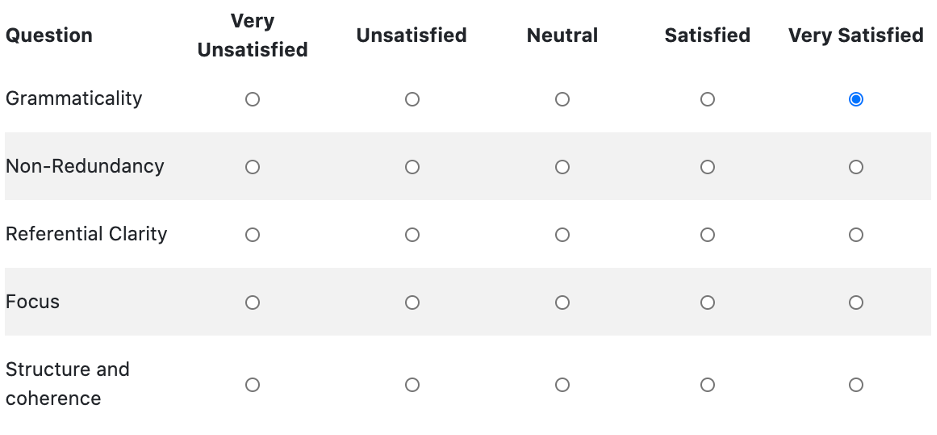
\includegraphics[scale=0.9]{content/pics/Picture_9.png}
\caption{ Potenziell mögliche Befragung, eigener Entwurf in Anlehnung an \cite{Dang}}
\label{Abbildung:Dang}
\end{figure}

In Abschnitt 4.3 werden zwei Verfahren zur Erzeugung von Zusammenfassungen evaluiert.


\section{Verfahren zur automatisierten Schnittstellen-Erkennung}

Dieser Anwendungsfall bezieht sich auf die Erkennung von Schnittstellen (Engl.: Interfaces). Gesucht sind technische Schnittstellen, die Abhängigkeiten zwischen einzelnen Anwendungen darstellen. Das Problem bei der Erkennung einer Schnittstelle anhand von Text in Englischer Sprache ist, dass das Vorkommen des Worts Interface alleine noch nicht unbedingt bedeutet, dass eine technische Schnittstelle identifiziert wurde. Es muss dabei mindestens unterschieden werden zwischen Technischen Schnittstellen (Technical Interfaces, Abk.: TI) und Benutzerschnittstellen (User Interfaces, Abk.: UI). Wenn Schnittstellen automatisch erkannt werden, dann können Sie anschließend visualisiert, etwa wie im Beispiel in Abbildung \ref{Abbildung:Interface_Circle} werden und entsprechend bei Entscheidungen im APM berücksichtigt werden. Das ist der große Mehrwert dieses Ansatzes. Zwei verschiedene Verfahren zur Lösung dieses Anwendungsfalls werden evaluiert in Kapitel 4.4.

\begin{figure}[h]
\centering
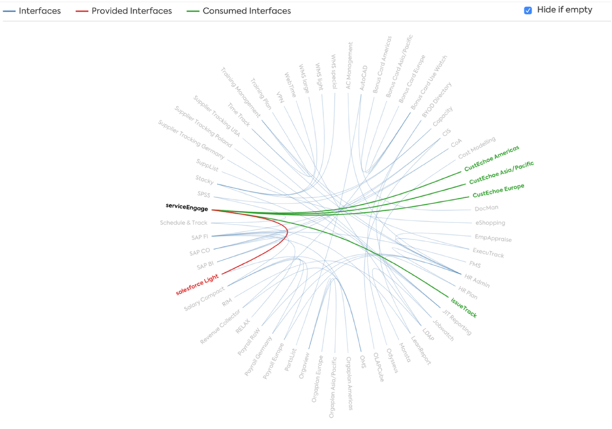
\includegraphics[scale=1.0]{content/pics/Picture_10.png}
\caption{ Schnittstellen-Visualiserung (Interface Circle Map) aus LeanIX, aus \cite{leanix2} }
\label{Abbildung:Interface_Circle}
\end{figure}

Alternativ zu Schnittstellen könnten mit derartigen Verfahren auch beispielsweise Anforderungen als solche klassifiziert werden, d.h. einzelne Sätze würden der Klasse Anforderungen zugeordnet. Sinnvoll im Kontext der IT-Governance ist das Erkennen einer Anforderung innerhalb eines Dokuments dann, wenn es z. B. einen dokumentierten Test für jede Anforderung geben muss. Dann könnte diese Überprüfung auf den durch ML erkannten Anforderungen aufbauen \cite{Vogelsang}. Hier könnte z. B. zwischen funktionalen und nicht-funktionalen Anforderungen unterschieden werden.

Statt den Klassen zur Schnittstellenerkennung könnten also auch andere Klassen verwendet werden. In Kapitel 4.4 erfolgt jedoch eine Begrenzung auf die Schnittstellen-Erkennung.

\section{Zu untersuchende Kriterien}

Einzelne Kennzahlen zur Bewertung von Ergebnissen sind wichtig für die Kommunikation von Ergebnissen an Projektbeteiligte. Hier werden nun Kriterien aufgestellt, anhand derer die Evaluation in dieser Arbeit durchgeführt werden soll. Die Kriterien sind:

\begin{itemize}
  \item Kriterium 1: Einsetzbarkeit der Methode unter den gegebenen Randbedingungen. Für die Evaluation von Verfahren standen bis zu 40 Text-Dokumente (im .docx-Format) zur Verfügung. Es soll überprüft werden, ob die jeweiligen Verfahren mit dieser recht geringen Datenmenge sinnvoll nutzbar sind und einen Mehrwert für das APM erbringen können. Wo es sinnvoll ist, können Metriken wie Accuracy, Precision, Recall, und die F1-Metrik eingesetzt werden.
  \item Kriterium 2: Generelle Einsetzbarkeit im APM-Kontext, unter der Annahme einer beliebig großen Datenmenge. Auch hier können entsprechende Metriken eingesetzt werden. 
  \item Kriterium 3: Vertretbarer Rechenaufwand der Methode. Untersucht werden hier z. B. die Dauer für das Training von Modellen, die Dauer zur Ausführung von Schätzungen, etc.
  \item 
Kriterium 4: Anfallende Kosten, welche zum Beispiel durch notwendige Lizenzierung von Modellen entstehen. Kosten können in der Praxis auch entstehen für das Zusammenstellen und Auszeichnen von Trainingsdaten, was durch Menschen geschehen muss. Es könnte auch sein, dass bei Einsatz gewisser Methoden oder bei Nutzung von großen Modellen eine bestimmte Hardware vorausgesetzt wird. 
\end{itemize}



\chapter{Ergebnisse der Evaluation}
\label{chap4}

Dieses Kapitel diskutiert die vier in Kapitel 3 definierten Anwendungsfälle sowie die ausgewählten Verfahren, die für die Realisierung der Anwendungsfälle in Frage kommen. Zusammengefasst wurden vier Anwendungsfälle identifiziert (vgl. Kapitel 3.1-3.4), für deren Implementierung in diesem Kapitel bestimmte Verfahren näher evaluiert werden. Die Anwendungsfälle sind:

\begin{enumerate}
  \item Ermittlung von Ähnlichkeiten
  \item Bestimmung von inhaltlicher Integrität
  \item Automatisierte Erzeugung von Text-Zusammenfassungen
  \item Automatisierte Schnittstellen-Erkennung
\end{enumerate}

Es werden für jeden Anwendungsfall nachfolgend jeweils zwei verschiedene Ansätze näher untersucht. Alle Ansätze werden anhand der in Kapitel 3.5 definierten Kriterien untersucht.

Die Testdaten stammen vom Auftraggeber. Es konnten bis zu 40 Dokumente (.docx-Format) verwendet werden, wobei in einzelnen Fällen auch Dokumente entfernt wurden, z. B. aufgrund von mangelnder Eignung der Inhalte für die Verfahren. 

\section{Ergebnisse: Ermittlung von Ähnlichkeiten}

Lösungsansatz 1 für diesen Anwendungsfall verwendet einen Ansatz auf Basis von Wort-Vektoren (vortrainierte spaCy-Vektoren). Ansatz 2 basiert ebenfalls auf Wort-Vektoren, es wird jedoch der Paragraph-Vector-Ansatz untersucht. Eine Visualisierung der Vektoren im zweidimensionalen Raum in Abbildung \ref{Abbildung:wordvecintuition} zeigt die Intuition hinter Wort-Vektoren. Die Vektoren aus der Abbildung wurden mit dem Verfahren Word2Vec mit Hilfe der Bibliothek gensim erzeugt. Die hochdimensionalen Wortvektoren wurden per Hauptkomponentenanalyse (Engl.: Principal Component Analysis, Abk.: PCA)  auf eine zweidimensionale Darstellung reduziert. Die Qualität der Vektoren kann etwa über Analogien evaluiert werden, wie ``Frau zu König ist wie Mann zu …`` \cite{rehurek2}, wobei man sich eigene Analogien ausdenken müsste, die im jeweiligen Kontext sinnvoll sind. Das ist eine Überlegung, die nicht weiter verfolgt wurde. Sie wird erwähnt, um klarzustellen, wie die Güte von selbst erstellten Vektoren zukünftig evaluiert werden könnte. 

\begin{figure}[]
\centering
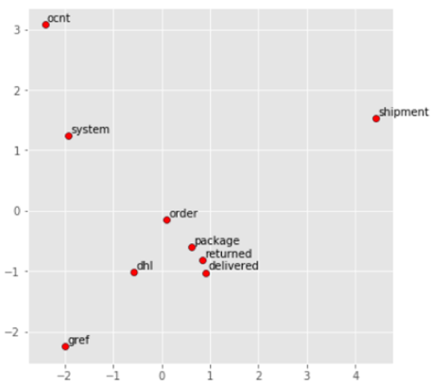
\includegraphics[scale=0.9]{content/pics/Picture_11.png}
\caption{Darstellung verschiedener Wörter in 2 Dimensionen , eigene Erstellung (Systemnamen wurden geschwärzt).}
\label{Abbildung:wordvecintuition}
\end{figure}

Abbildung \ref{Abbildung:wordvecintuition} basiert auf einem eigenen Experiment, in dem die verfügbaren Kunden-Dokumente in Kleinschreibung (etwa 330 000 Wörter; entspricht einer Größe von 2.1 Megabyte) für das Training eines eigenen Wort-Vektor-Modells verwendet wurden. Das so erzeugte Modell hat zwar spezielle Begriffe (etwa die Namen von einzelnen Projekten) aus den Dokumenten gelernt, es hat aber z. B. keine Idee davon, wie beliebige Begriffe wie ``London`` oder ``Paris`` einzuordnen sind. Diese Begriffe sind nicht einmal Teil des Vokabulars. Das zeigt, dass ein selbst trainiertes Modell nur bedingt für den Vergleich von Dokumenten geeignet ist. Es kann geschlussfolgert werden, dass das Training eines geeigneten Modells domänenspezifische Dokumente und zusätzlich einen ``allgemeinen`` Textkorpus voraussetzen würde, damit sinnvoll mit dem Modell gearbeitet werden könnte. Perspektivisch könnte also ein solches fortgeschrittenes Modell trainiert werden. 

\subsection{Ansatz 1: Ähnlichkeitsvergleich mit einem Word2Vec-Modell}

Im nachfolgenden, einleitenden Beispiel wurde die Ähnlichkeit zwischen ganzen Dokumenten berechnet. 
Aufgrund der beschriebenen Schwierigkeiten mit einem selbst trainierten Modell wird hier für die Evaluation das vortrainierte, gebrauchsfertige Wort-Vektor-Modell von spaCy verwendet. Es wurde das größte verfügbare Modell \(en\_core\_web\_lg\) gewählt. Das Modell deckt von den Begriffen aus den Kundendokumenten lediglich 91,9 Prozent der Begriffe durch Vektoren ab. Das heißt, es gibt für 8,1 Prozent der Begriffe in den Kundendokumenten keine Vektoren in dem gebrauchsfertigen spaCy-Modell\footnote{Berechnung: Wörter die keinen spaCy-Vektoren besitzen/ Gesamtanzahl der Wörter aus den Dokumenten}. Aus diesem Grund steht bereits an dieser Stelle fest, dass ein gebrauchsfertiges Modell für die Berechnung von Ähnlichkeiten recht viele wichtige Begriffe nicht berücksichtigen kann. Abbildung \ref{Abbildung:listing_1} zeigt exemplarisch, wie die Ähnlichkeit von Texten in Python auf Basis von Wort-Vektoren ermittelt werden kann. Das dargestellte Skript liefert ein Ähnlichkeitsmaß von 0.98. Es handelt sich in dem Beispiel um Dokumente, die unterschiedliche Versionen der gleichen Software beschrieben. Der gleiche Test mit doc1 aus der Abbildung und einem Dokument aus einem anderen Projekt lieferte eine Punktzahl von 0.951064. Grundsätzlich sind die Ausgaben also interpretier- und nachvollziehbar. Für das APM heißt das, dass durchaus sprachlich verwandte Dokumente und damit potenziell ähnliche Anwendungen identifziert werden können, wie im Folgenden noch weiter gezeigt wird. Zu beachten bei den Ergebnissen oben ist stets, dass einige domänenspezifische Wörter bei diesem verwendeten Modell keine Vektoren besitzen und deshalb gar nicht berücksichtigt werden können, wie bereits angedeutet. Eine Option zur Lösung des Problems bestünde darin, Vektoren komplett neu zu trainieren. 

\begin{figure}[h]
\centering
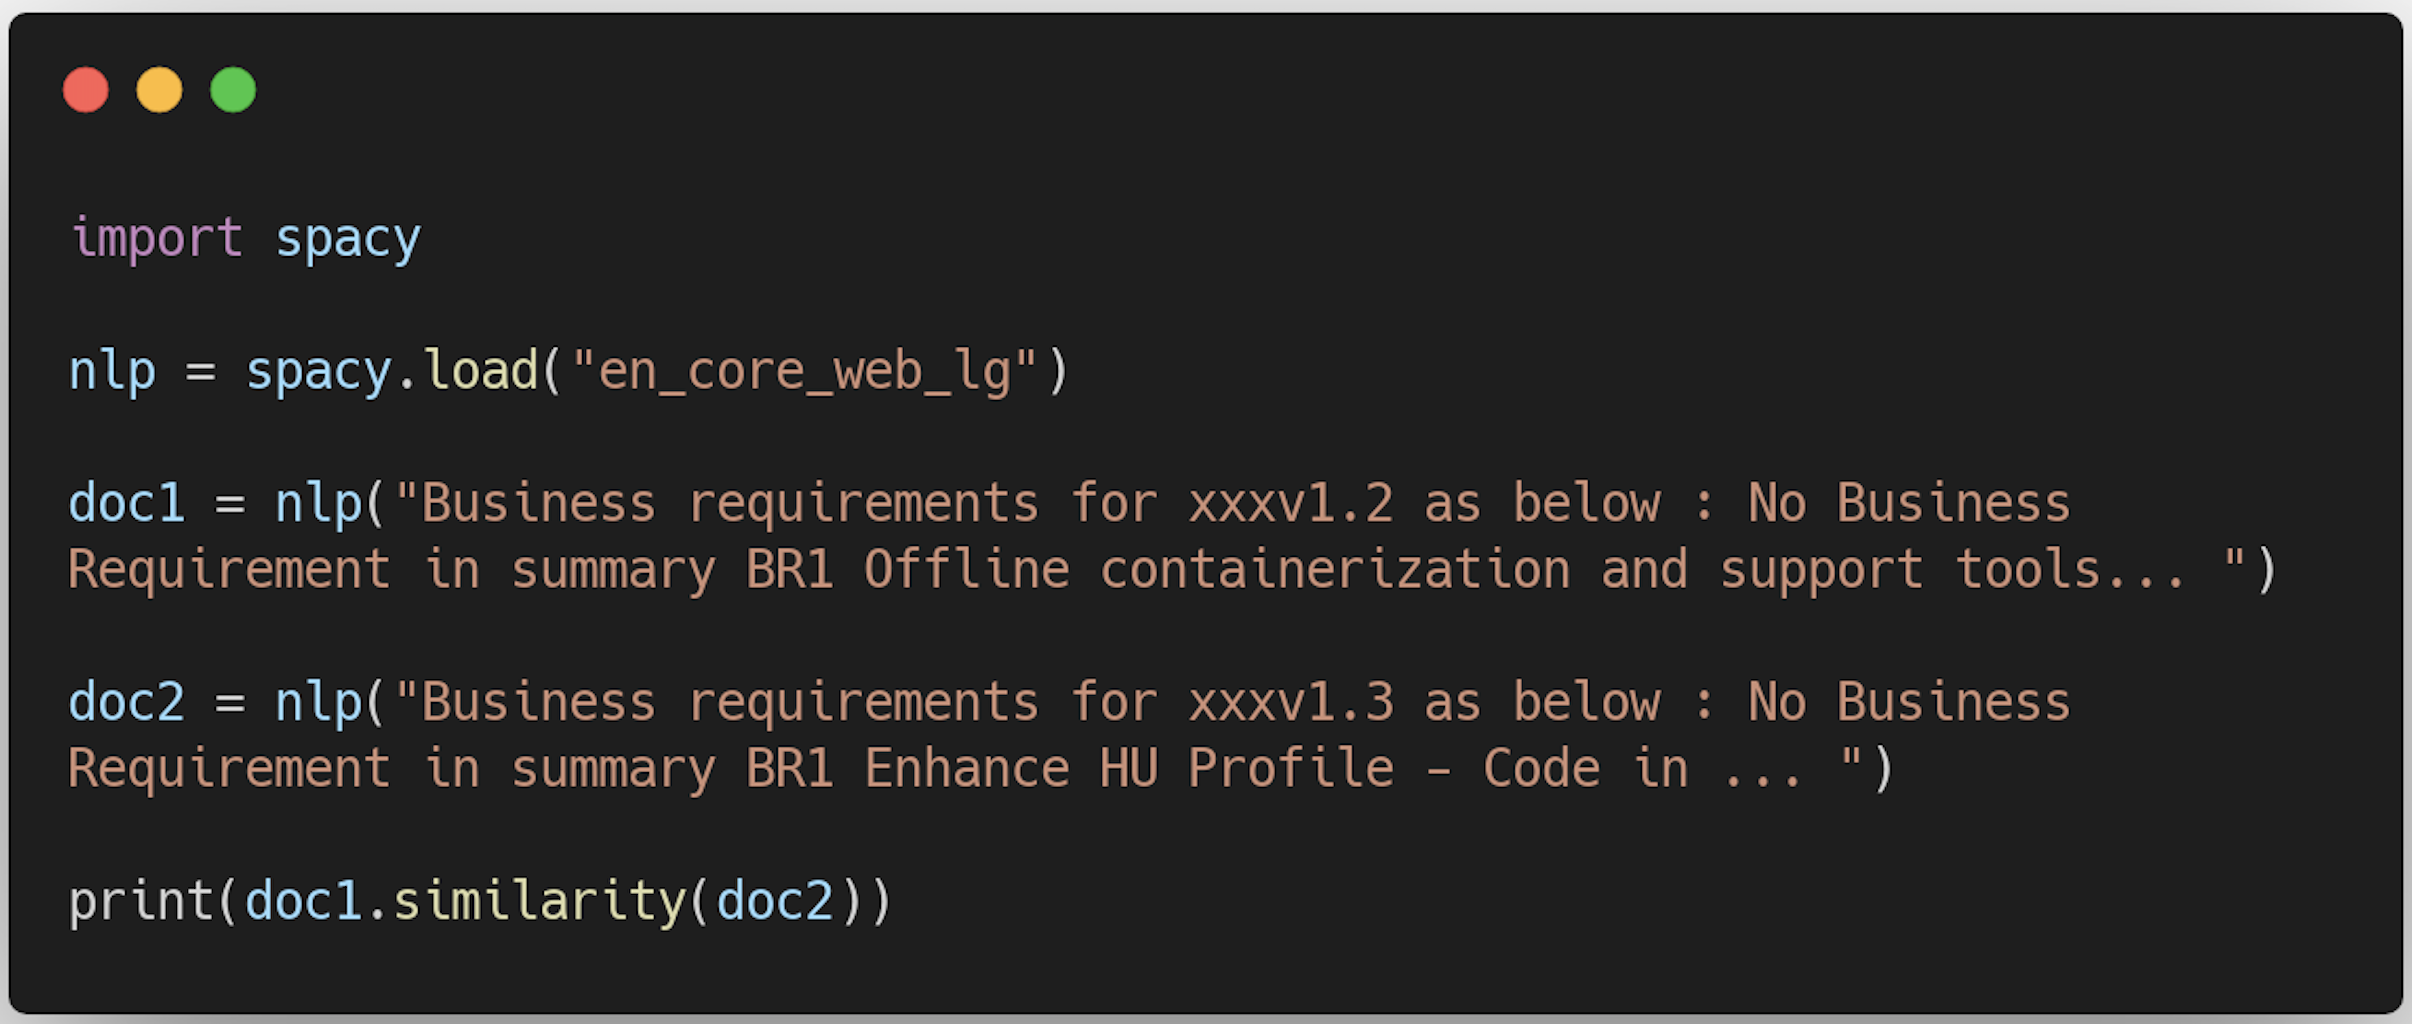
\includegraphics[scale=0.35]{content/pics/Listing_1_.png}
\caption{Similarity Berechnung mit spaCy. Die Texte wurden gekürzt.}
\label{Abbildung:listing_1}
\end{figure}

{\bf Kriterium 1: Einsetzbarkeit des Ansatzes unter den gegebenen Rahmenbedingungen}

Unten dargestellt (Abbildung \ref{Abbildung:heatmap1}) ist eine Heatmap, welche die Ähnlichkeit von Dokumenten zueinander visualisiert. Aus Datenschutzgründen werden hier nicht die Namen der Dokumente, sondern interne IDs präsentiert. In diesem Versuch wurden keine Stoppworte entfernt. Das erklärt, weshalb die Skala lediglich von 1 (zu interpretieren als ``Dokumente sind vollständig identisch``) bis 0,95 (zu interpretieren als ``Dokumente sind sich sehr ähnlich``) verläuft. In Abbildung \ref{Abbildung:heatmap2} ist das Ergebnis beim gleichen Vorgehen mit Stoppwortentfernung dargestellt. Die Skala verändert sich, d. h. Dokumente sind sich weniger ähnlich als vorher. Insgesamt sind aber kaum Unterschiede zu oben (Abbildung \ref{Abbildung:heatmap1}) erkennbar. 
 
\begin{figure}[h]
\centering
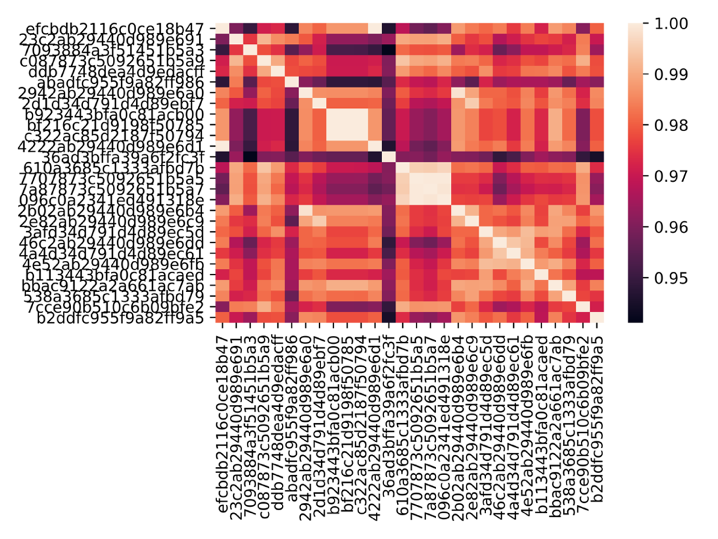
\includegraphics[scale=0.95]{content/pics/Picture_12.png}
\caption{Heatmap zur Dokumentenähnlichkeit, eigene Erstellung}
\label{Abbildung:heatmap1}
\end{figure}

\begin{figure}[h]
\centering
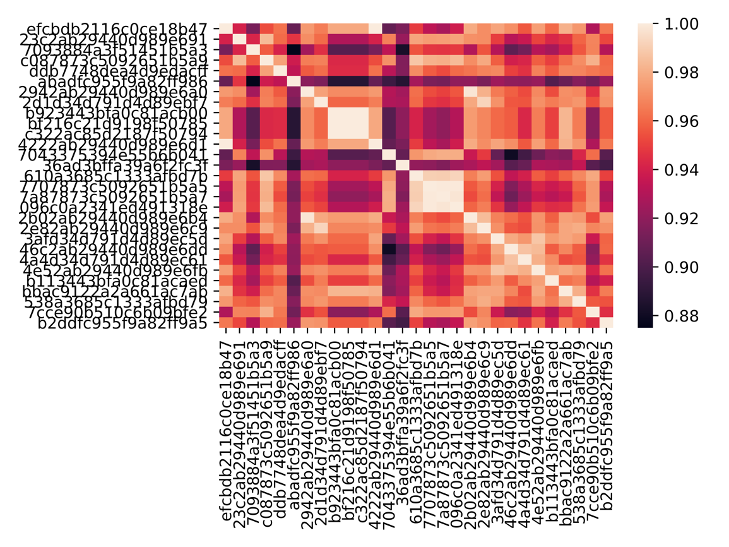
\includegraphics[scale=0.95]{content/pics/Picture_13.png}
\caption{Heatmap zur Dokumentenähnlichkeit, mit Stoppwortentfernung, eigene Erstellung}
\label{Abbildung:heatmap2}
\end{figure}

Es sind weitere Verfeinerungen denkbar, wie die Entfernung aller Verben oder Adjektive, oder die manuelle Gewichtung von bestimmten Substantiven. Ein solches Vorgehen geht in Richtung regelbasierte Sprachverarbeitung und wird daher hier nicht weiterverfolgt. 

Der Ansatz ist also mit der gegebenen Datenmenge (20-40 Dokumente) sinnvoll einsetzbar, auch wenn durch ein Training eigener Vektoren noch Verbesserungen im Hinblick auf die Ergebnisse zu erwarten sind. Er liefert zumindest Hinweise darauf, in welchen Dokumenten bzw. Projekten mit ähnlicher Sprache gearbeitet wird.
Die Metrik (etwa ``Ähnlichkeit von 0,99``) kann zum Beispiel genutzt werden, um zu überprüfen, ob ein Dokument anderen existierenden Dokumenten ähnelt. Ein Entscheider könnte sich dieses ähnliche Dokument dann noch einmal genauer ansehen, um zu prüfen, ob beispielsweise Systeme mit ähnlichen Anforderungen entdeckt wurden.

{\bf Kriterium 2: Generelle Einsetzbarkeit des Ansatzes im APM-Kontext, unter der Annahme einer beliebig großen Datenmenge}

Für Kriterium 2 gilt das gleiche wie bei Kriterium 1. Eine größere Datenmenge würde das Training eines eigenen, auf den IT-Governance-Kontext zugeschnittenen Vektor-Modells ermöglichen, wodurch noch genauere Ergebnisse zu erwarten wären.

{\bf Kriterium 3: Rechenaufwand}

Das Vergleichen von nur zwei Dokumenten mit durchschnittlich 5000 Wörtern dauert auf gewöhnlicher Hardware bereits einige Sekunden. Bei 30 Dokumenten würden sich 900 durchzuführende Vergleiche ergeben (870 wenn man Dokumente nicht mit sich selbst vergleicht). 

Von der Komplexitätsklasse ist das ein quadratisches Problem: 
$\mathcal{O}(n^2)$, wenn $n$ die Anzahl der Dokumente ist. 

Es ist also mit einer gewissen Dauer zu kalkulieren, wenn die Ähnlichkeit dynamisch berechnet werden sollte. Die Ähnlichkeit von einzelnen Dokumenten zueinander wird berechnet auf Basis der Kosinus-Ähnlichkeit, wobei zunächst von allen Vektoren der jeweiligen Dokumente der Durchschnitt berechnet wird \cite{spacy3}. Die Kosinus-Ähnlichkeit ermittelt einen Wert zwischen -1 und 1 für die Ähnlichkeit von zwei Vektoren A und B \cite[S. 84]{Gupta}:	
 
 \begin{equation}
similarity = {{\bf A} \times {\bf B} \over \|{\bf A}\| \|{\bf B}\|} = \frac{ \sum_{i=1}^{n}{{\bf A}_i{\bf B}_i} }{ \sqrt{\sum_{i=1}^{n}{({\bf A}_i)^2}} \sqrt{\sum_{i=1}^{n}{({\bf B}_i)^2}} }
\end{equation}

Der Rechenaufwand zur Erzeugung der fachspezifischen Vektoren ist abhängig von der Größe des jeweiligen Trainingskorpus. 
%\\
%\\
% \\ 

{\bf Kriterium 4: Kosten}

Es sind hier keine Kosten durch Lizensierung oder manuelle Tätigkeiten erkennbar, zumindest solange, wie mit den vortrainierten Wort-Vektoren gearbeitet wird. spaCy-Modelle verwenden die MIT-Lizenz \cite{spacy-license}, welche die kostenfreie Nutzung ermöglicht \cite{MIT}. Wenn ein Textkorpus zusammengestellt werden sollte, um eigene Vektoren zu erzeugen, dann müssten entsprechende Dokumente aus unterschiedlichen Quellen gesammelt werden, was Aufwand bedeuten würde.


\subsection{Ansatz 2: Ähnlichkeitsvergleich unter Verwendung des Paragraph-Vector-Modells (Doc2Vec)}

Das Paragraph-Vector-Modell kann ebenfalls für die Ermittlung von Ähnlichkeiten von Dokumenten eingesetzt werden \cite{Dai}. Nachfolgend wird dieses Verfahren im Kontext des APM zur Ermittlung von ähnlichen Dokumenten untersucht. Die Ähnlichkeit zwischen Dokumenten kann abgesehen von einer Heatmap (wie im vorangegangenen Abschnitt) auch über Cluster in einem Streudiagramm visualisiert werden. Diese Form der Visualisierung wird hier gewählt. Dokumente die sich ähneln, würden im Streudiagramm nahe beieinander liegen, wie nachfolgend gezeigt wird. 

{\bf Kriterium 1: Einsetzbarkeit des Ansatzes unter den gegebenen Rahmenbedingungen}

Es wird hier ein eigenes Doc2Vec-Modell trainiert. Das Verfahren Doc2Vec von gensim erzeugt für jedes Dokument einen Vektor. Diese Vektoren können je nach Parameterwahl verschiedene Dimensionen haben. Um die Vektoren in einer zweidimensionalen Ebene darstellen zu können, wurde t-SNE (t-Distributed Stochastic Neighbor Embedding, nach \cite{t-SNE}) zur Dimensionsreduktion verwendet. Es wurde davon ausgegangen, dass ähnliche Dokumente auch ähnliche Vektoren haben. Dadurch sollten in Abbildung \ref{Abbildung:doc2vec1} Cluster erkennbar sein – wie nachfolgend unter Kriterium 2 beschrieben – dies ist jedoch hier zunächst nicht der Fall. Das Verfahren eignet sich also in der Variante, die hier evaluiert wurde, nicht für den Einsatz bei einer derart kleinen Datenmenge. Ein Punkt stellt ein Dokument dar, die Farbe zeigt den Dokumententyp des Dokuments. Auf eine Beschriftung der einzelnen Datenpunkte wird aus optischen Gründen sowie aus Datenschutzgründen verzichtet. Es wurde erwartet, dass Dokumente des gleichen Dokumententyps Cluster bilden würden (vgl. die Ausführungen unter Kriterium 2)

\begin{figure}[h]
\centering
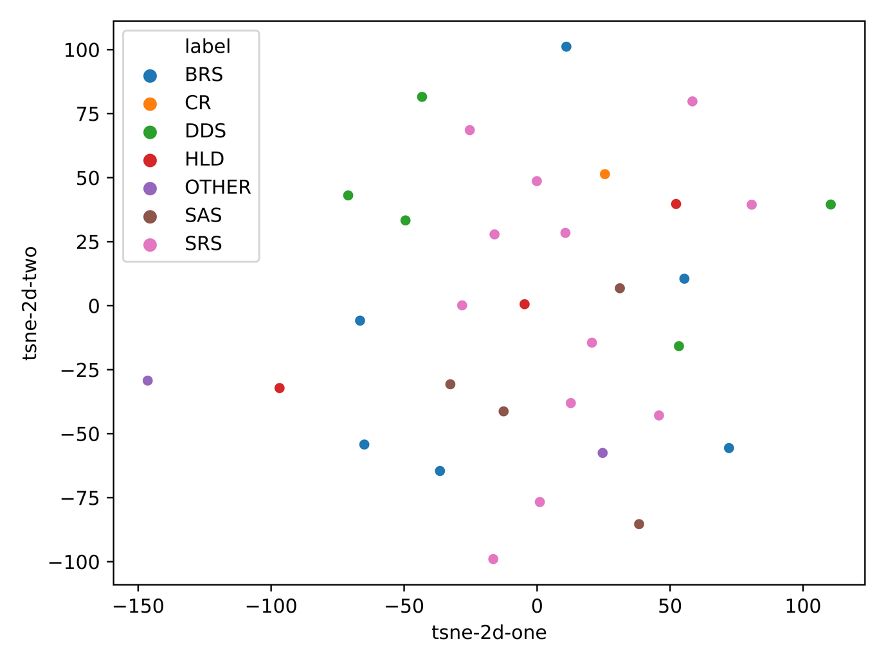
\includegraphics[scale=0.95]{content/pics/Picture_14.png}
\caption{Darstellung aller verfügbaren Dokumente, gruppiert nach Dokumententypen, eigene Erstellung}
\label{Abbildung:doc2vec1}
\end{figure}

Die Achsenbeschriftungen der Abbildung \ref{Abbildung:doc2vec1} ergeben sich lediglich durch die Dimensionsreduktion und haben keine besondere Bedeutung.

Für das APM geschlussfolgert wird, dass auch die Suche nach Dokumenten-Clustern (Anwendungs-Cluster) hilfreich sein könnte. Mit Doc2Vec und der Dimensionsreduktion kann derartiges erreicht werden, jedoch sind dazu insbesondere weitere Textdokumente notwendig.

{\bf Kriterium 2: Generelle Einsetzbarkeit des Ansatzes im APM-Kontext, unter der Annahme einer beliebig großen Datenmenge}

Man kann mit dem Verfahren grundsätzlich Cluster bilden. Dies belegt ein Beispiel aus der Literatur, auf das hier eingegangen wird. Die Dimensionsreduktion erfolgte ebenfalls mit t-SNE (vgl. Abbildung \ref{Abbildung:doc2vec2}) \cite{Dai}. 

Es werden in dem Beispiel ähnliche Wikipedia-Artikel zu Dokumenten-Clustern zusammengefasst, wodurch die generelle Einsetzbarkeit unter der Annahme einer beliebig großen Menge von Dokumenten bestätigt werden kann. Es kann allerdings nicht ausgeschlossen werden, dass die APM-Dokumente sich nicht genug voneinander unterschieden, womit das Wikipedia-Ergebnis im Kontext des APM nicht erzielt werden könnte. 

In einer realen Anwendung könnte sich z. B. durch das Auswählen einzelner Datenpunkte ein Fenster mit Details zum jeweiligen Dokument öffnen. Im Falle eines neuen Dokuments könnte die Position in der Visualisierung Hinweise darauf geben, welche ähnlichen Dokumente (bzw. Anwendungen) es bereits gibt. 

\begin{figure}[h]
\centering
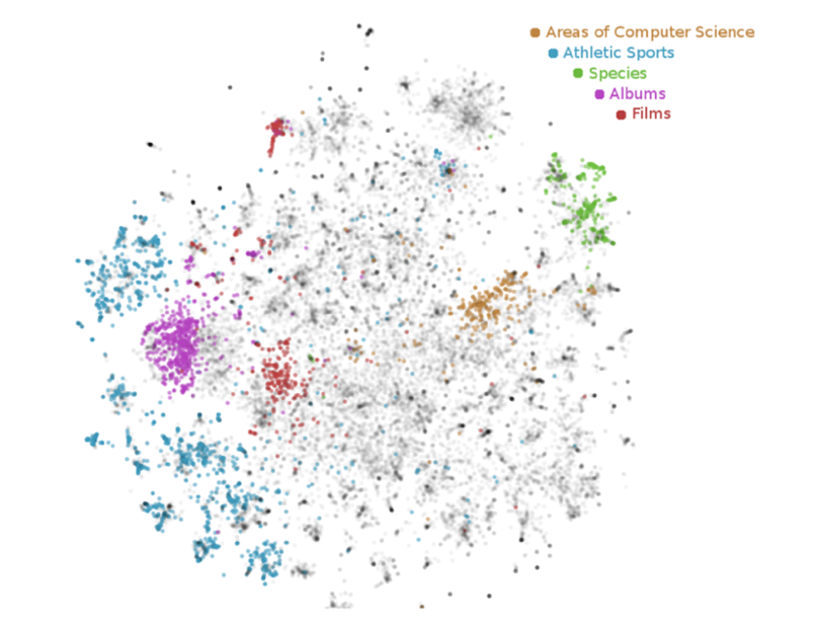
\includegraphics[scale=0.95]{content/pics/Picture_15.png}
\caption{Wikipedia-Dokumenten-Cluster, gruppiert nach Kategorien, erzeugt über Doc2Vec, aus \cite{Dai}}
\label{Abbildung:doc2vec2}
\end{figure}

%\smallskip

{\bf Kriterium 3: Rechenaufwand}

Das Erzeugen eines Scatter-Plots wie in Abbildung \ref{Abbildung:doc2vec2} erfordert zunächst das Training eines Modells. Die Trainingszeit ist abhängig von der Anzahl der Dokumente. Ein solches Modell kann auch nachts trainiert werden und dann gespeichert werden. Neue Dokumente können dann durch das Modell in Vektorform gebracht und visualisiert werden, z. B. in einer interaktiven Darstellung etwa auf einer Webseite. Die Inferenz (Erzeugung von Dokumenten-Vektoren) erfolgt ohne Verzögerungen.

{\bf Kriterium 4: Kosten}

Der Paragraph-Vector-Ansatz benötigt keine beschrifteten Beispiele und kann daher auch in Szenarien eingesetzt werden, in denen es keine beschrifteten Daten gibt \cite[S. 4]{mikolov2014}. Daher ist für das Erzeugen von Beschriftungen kein manueller Aufwand nötig, der Kosten verursachen würde. Der Ansatz benötigt dennoch aufbereitete Dokumente für das Training eines Modells. Diese sind zusammenzustellen. Lizenzkosten gibt es bei der Verwendung der Bibliothek gensim nicht \cite{gensim-license}.

\section{Ergebnisse: Bestimmung von inhaltlicher Integrität}

Bei der ``Bestimmung von inhaltlicher Integrität`` wird der Inhalt von einzelnen Kapiteln aus Anwendungsdokumentationen betrachtet. Dieser soll idealerweise das beschreiben, was erwartet wird. In einem Kapitel zu (beispielsweise) ``Anforderungen`` soll es auch um Anforderungen gehen, und nicht um etwas anderes.

\subsection{Ansatz 1: Vergleich von Durchschnitts-Wort-Vektoren}

Dieser Ansatz basiert auf durchschnittlichen Wort-Vektoren. Auf Basis einer Trainingsdatenmenge werden zunächst durchschnittliche Wort-Vektoren berechnet. Die Trainingsdatenmenge setzt sich zusammen aus mehreren Textkörpern. Die unterschiedlichen Textkörper bestehen hier aus frei zugänglichen PDF-Dokumenten aus dem Internet. Unterschieden werden dabei die folgenden Dokumententypen:

\begin{itemize}
\item Texte, in denen Anforderungen beschrieben werden (Thema Requirements)
\item Texte zu Lösungs-Architekturen (Thema Architecture bzw. Architectural Language)
\item Texte zu Software-Design (Thema Design) 
\item Texte zu Logistik-Themen (Thema Logistics)
\end{itemize}

Für jeden dieser Typen wird ein durchschnittlicher Wort-Vektor berechnet. Visualisiert wird das Vorgehen in Abbildung \ref{Abbildung:avgvec}. Nicht gezeigt wird hier der Logistik-Textkorpus.

\begin{figure}[h]
\centering
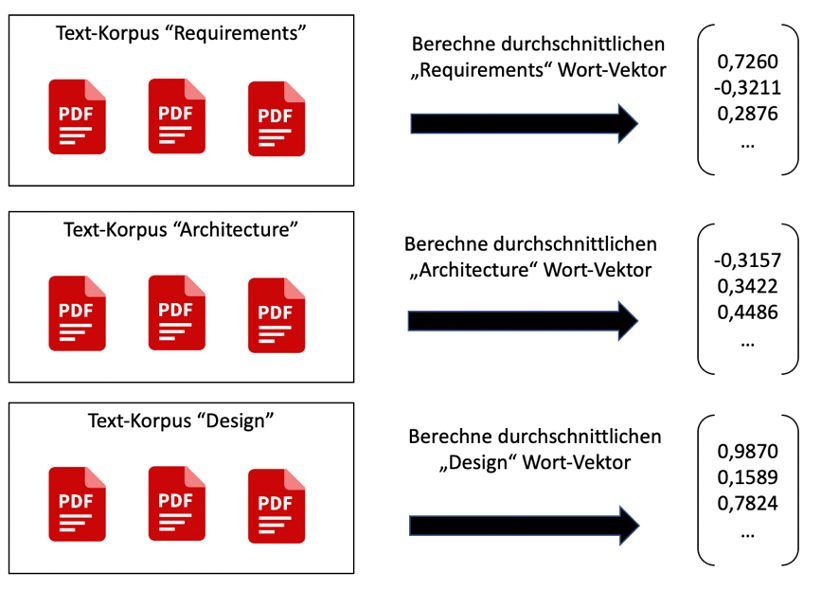
\includegraphics[scale=0.95]{content/pics/Picture_16.png}
\caption{Initiale Vorbereitung von durchschnittlichen Wort-Vektoren, eigene Erstellung}
\label{Abbildung:avgvec}
\end{figure}

Ziel ist es nun auf Kapitelebene zu schätzen, ob es in einzelnen Kapiteln von Test-Dokumenten um eines der festgelegten Themen (Requirements, Architectural Language, Design oder Logistics) geht, wie in Kapitel 3.2 beschrieben. Das Thema Logistik dient dabei als Referenz- bzw. als Vergleichskorpus. Hintergrund ist stets die Prüfung, ob ein Kapitel enthält, was es laut Vorgabe enthalten sollte. Die Zielvariable heißt ``erkanntes Thema`` – sie kann verwendet werden, um die Wahrscheinlichkeit zu messen, mit der ein Kapitel die erwarteten Inhalte enthält. Die Wahrscheinlichkeiten ergeben sich, indem für jedes Kapitel in einem zu untersuchenden Beispiel-Dokument ebenfalls Vektoren erzeugt werden. Diese werden dann mit den Durchschnitts-Vektoren verglichen (vgl. Abbildung \ref{Abbildung:avgvec2}). 

\begin{figure}[h]
\centering
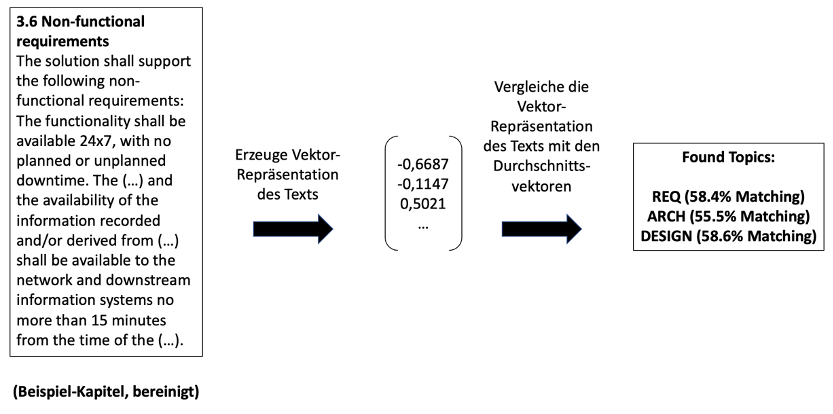
\includegraphics[scale=0.95]{content/pics/Picture_17.png}
\caption{Inferenz-Phase. Vergleich von Kapitel-Vektoren mit Durchschnitts-Vektoren, eigene Erstellung}
\label{Abbildung:avgvec2}
\end{figure}

{\bf Kriterium 1: Einsetzbarkeit des Ansatzes unter den gegebenen Rahmenbedingungen}

Als Trainingsmenge können beliebig viele Dokumente verwendet werden. Hier wurden pro Text-Korpus etwa 20 PDF-Dokumente aus dem Internet verwendet. Auf Basis dieser Dokumente wurden die Durchschnittsvektoren ermittelt. 
In Abbildung \ref{Abbildung:avgvec2} werden mögliche Resultate schon angedeutet. Die Schätzungen haben meist mit mehreren Durchschnittsvektoren Ähnlichkeiten. Daher kann hier von keiner zuverlässigen Vorhersage der Topics gesprochen werden. 
Es werden hier auch keine Metriken im Sinne einer Konfusionsmatrix präsentiert, weil Abschnitte stets mit mehreren der Topics eine Ähnlichkeit hatten. Das zeigt auch der nachfolgende direkte Vergleich von den durchschnittlichen Vektoren (vgl. Tabelle \ref{table:4}).

\begin{table}[h]
\centering
\begin{tabular}{|c|c|c|c|c|}
\hline
                      & \textbf{Logistics} & \textbf{Architecture} & \textbf{Design} & \textbf{Requirements} \\ \hline
\textbf{Logistics}    & 1                  & 0.93                  & 0.91            & 0.92                  \\ \hline
\textbf{Architecture} & 0.93               & 1                     & 0.99            & 0.98                  \\ \hline
\textbf{Design}       & 0.91               & 0.99                  & 1               & 0.99                  \\ \hline
\textbf{Requirements} & 0.92               & 0.98                  & 0.99            & 1                     \\ \hline
\end{tabular}
\caption{Vergleich der Durchschnitts-Vektoren miteinander. Der Vergleich erfolgte mit der Similarity-Funktion von spaCy.}
\label{table:4}
\end{table}

Als Ursache für die Ähnlichkeit der Vektoren (mit Ausnahme des Referenzkorpus ``Logistics``, wo durchaus eine Unterscheidung möglich ist) wird von der inhaltlichen Nähe der Text-Körper zueinander ausgegangen (vgl. etwa ``Design`` und ``Architecture``, wo eine Ähnlichkeit von 0,99 gegeben ist, die Vektoren also beinahe gleich sind. Bei Vergleichen mit ``Logistics`` ist eine derart starke Ähnlichkeit nicht gegeben). Die gewählten Topics sind sich inhaltlich sehr ähnlich, weshalb hier die sorgfältige Auswahl der Trainingsdokumente in den jeweiligen Kategorien eine Rolle spielt. Die einfache Durchschnittsbildung (averaging) führt also im Kontext des APM eher weniger zu sinnvollen Vektoren, weshalb mit einer derart geringen Datenmenge der Ansatz nicht sinnvoll genutzt werden kann.
Aus den Ergebnissen folgt jedoch, dass man mit dem Verfahren zumindest ein Gefühl dafür bekommen kann, ob die Inhalte einzelner Kapitel grob in die richtige Richtung gehen. Texte wie etwa {\textit{lorem ipsum}}, könnten als unsinnige Inhalte identifiziert werden.

{\bf Kriterium 2: Generelle Einsetzbarkeit des Ansatzes im APM-Kontext, unter der Annahme einer beliebig großen Datenmenge}

Wie oben beschrieben (vgl. Tabelle \ref{table:4}), sind die gewählten Themen, mit Ausnahme des Themas Logistics, sich inhaltlich sehr ähnlich. Das ändert sich auch bei größeren Trainingsdatenmengen nicht, da die Dokumente sich inhaltlich stets sehr ähnlich sein werden. Daher kann hier die generelle Einsetzbarkeit dieses Ansatzes nicht bestätigt werden, sofern zwischen sehr ähnlichen Themen (wie im vorliegenden Kontext) unterschieden werden soll.

Die Autoren dieser Studie \cite{dilawar} evaluierten ebenfalls verschiedene Ansätze zur Kombination von Wort-Vektoren, so wie es bis hierhin beschrieben wurde. Allerdings unterscheidet sich der Ansatz der Autoren darin, dass kein schlichter Vektor-Vergleich mit Durchschnittsvektoren durchgeführt wird. Stattdessen werden Vektor-Repräsentationen des Texts noch als Eingabe für ein Klassifizierungsverfahren verwendet, wobei ein neuronales Netz zum Einsatz kommt. Dabei handelt es sich im Prinzip um einen eigenen Ansatz. Da es in diesem Abschnitt um den Vergleich von Durchschnitts-Vektoren ging, wird der Klassifizierungsansatz hier nicht näher betrachtet, er soll aber als Möglichkeit für weitere Versuche dokumentiert werden.


{\bf Kriterium 3: Rechenaufwand}

Ein gebräuchliches Maß zur Bewertung der Ähnlichkeit ist die Kosinus-Ähnlichkeit. Der eigentliche Abgleich der Vektoren erfolgt mit dieser Metrik, unter Verwendung der spaCy-Similarity-Funktion. Details zur Kosinus-Ähnlichkeit wurden bereits in Abschnitt 4.1.1 unter Kriterium 3 beschrieben. Als Wort-Vektoren wurden hier die vortrainierten Vektoren von spaCy genutzt. Daher ist kein Aufwand für das Training notwendig, sofern das vortrainierte Modell gewählt werden soll. Alternativ können Wort-Vektoren auch selbst trainiert werden, dann wäre ein entsprechender Rechen- und Zeitaufwand zu berücksichtigen.

{\bf Kriterium 4: Kosten}

Es können frei verfügbare Software-Bibliotheken (u. a. spaCy \cite{spacy-license}, NumPy \cite{numpy-license}) verwendet werden. Kosten entstehen durch das Sammeln und das Verwalten von Dokumenten für das Training. Im vorliegenden Beispiel wurden zunächst im Internet Dokumente als Ausgangsbasis für die Durchschnittsbildung gesucht, was aufwändig wird, wenn eine hohe Anzahl an Dokumenten mit ausreichender Qualität gesucht werden soll.

\subsection{Ansatz 2: Topic Modelling mit Non-negative matrix factorization}

Wie oben bereits angedeutet, gäbe es für die Lösung des Anwendungsfalls ``Bestimmung von inhaltlicher Integrität`` weitere Möglichkeiten aus den Bereichen des überwachten, unüberwachten oder auch semi-überwachten Lernens. Mit verschiedenen Klassifizierungsverfahren können die Klassen beziehungsweise die Themen von einzelnen Kapiteln aus Text-Dokumenten geschätzt werden. In Frage kämen etwa Ansätze wie Naive Bayes, logistische Regression, neuronale Netze, und andere. Hier vorgestellt wird nun ein Ansatz auf Basis von Non-negative matrix factorization (Abk.: NMF). Zu beachten ist, dass es sich dabei nicht um ein Klassifizierungsverfahren, sondern um eine Methode aus der Kategorie des Topic Modelling handelt. Statt mit NMF könnten ähnliche Resultate auch unter Verwendung des Verfahrens Latent Dirichlet Allocation (Abk.: LDA) realisiert und evaluiert werden \cite{scikit1}.

Als Trainingskorpus wird auch hier eine Menge von Dokumenten aus dem Internet verwendet. Verwendet wurden  wiederum die Textkorpora Requirements, Architectural Language, Design sowie Logistics. Bei näherer Betrachtung des Trainingskorpus fällt auf, dass die Trainingsdokumente in den einzelnen Kategorien sich durchaus durch bestimmte, typische Begriffe auszeichnen. Diese Begriffe sind die bedeutsamsten für ein bestimmtes Thema. Zur Visualisierung dieser Begriffe von Topics können Ansätze wie NMF oder LDA genutzt werden. Diese Ansätze verwenden intern als Vorverarabeitungsschritt die TF-IDF-Metrik. Zur Schätzung des Topics eines Testdokuments kann dann das erstellte Modell genutzt werden. Zunächst folgt allerdings in Abbildung \ref{Abbildung:word-clouds} eine Visualisierung der für die Themen typischen Begriffe. Die Begriffe die von Bedeutung sind für ein Thema wurden automatisch durch das Verfahren extrahiert und sind unten dargestellt.
 
\begin{figure}[h]
\centering
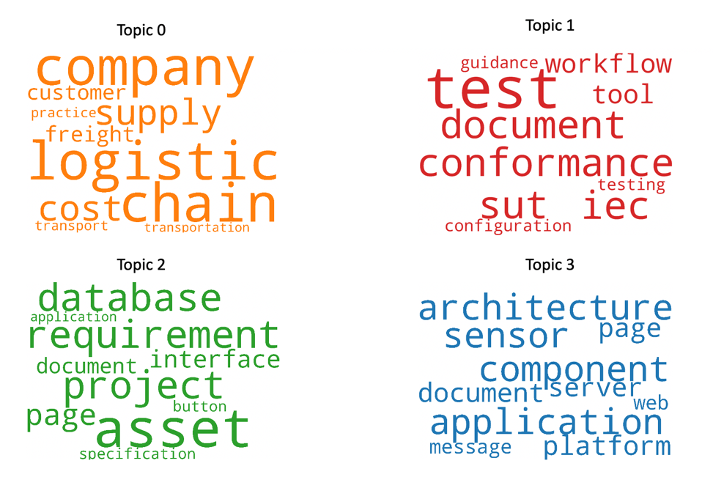
\includegraphics[scale=0.95]{content/pics/Picture_18.png}
\caption{Tag Clouds zu 4 erkannten Topics, erstellt mit NMF (eigene Erstellung)}
\label{Abbildung:word-clouds}
\end{figure}

Mit bloßem Auge erkennbar sind in Abbildung \ref{Abbildung:word-clouds} die Themen Requirements (Topic 2), Architectural Language (Topic 3) und Logistics (Topic 0). Für die Vorhersage des Topics eines neuen Dokuments (Testdokumente) werden noch weitere als die je 10 hier dargestellten Begriffe verwendet. Es handelt sich jedoch bei den Begriffen in Abbildung \ref{Abbildung:word-clouds} um jene Begriffe, die laut Modell am aussagekräftigsten für die Topics sind. Die Vorhersage des Themas eines Testdokuments liefert als Ergebnis eine Zuordnung zu einem der vier Themen. Ein Beispiel ist abgebildet in Abbildung \ref{Abbildung:nmf-inf}.

\begin{figure}[h]
\centering
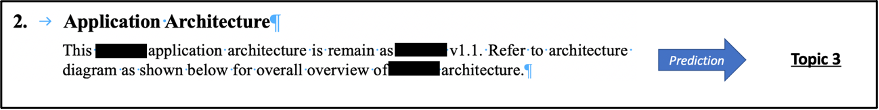
\includegraphics[scale=0.95]{content/pics/Picture_19.png}
\caption{Verwendung eines Abschnitts aus einem Testdokument für die Vorhersage des Topics, eigene Erstellung}
\label{Abbildung:nmf-inf}
\end{figure}
 
Dieses Verfahren sagt dem Nutzer lediglich, dass zum Beispiel Topic 3 als Ergebnis einer Vorhersage bestimmt wurde. Das Verfahren sagt nicht, wie das Topic zu interpretieren ist, also um welche ``Klasse`` es sich bei dem Topic handelt. Die ``Klassen`` müssen deshalb manuell auf Basis der Tag Clouds (Abbildung \ref{Abbildung:word-clouds}) bestimmt werden.

{\bf Kriterium 1: Einsetzbarkeit des Ansatzes unter den gegebenen Rahmenbedingungen}

Es wurden per Hand Text-Beispiele für Tests ausgewählt und entsprechende Beschriftungen erzeugt. Es wurden manuell 4 Texte dem Thema Software Design zugeordnet, 13 der Kategorie Requirements, und 3 wurden als Architectural Language eingeordnet. Für jedes Beispiel wird eine Schätzung mit dem NMF-Modell durchgeführt. Die Ergebnisse der Schätzungen sind unten (Tabelle \ref{tab:confusion-nmf}) dargestellt. Topic 0 (``Logistics``) kann als Kontroll-Klasse verstanden werden, die eigentlich nicht vorhergesagt werden sollte. Die Klasse ``Requirements`` könnte aus fachlicher Sicht auch in zwei Klassen functional und non-functional aufgeteilt werden. Diese Unterscheidung wurde hier nicht gemacht.

\begin{table}[h]
\centering
\begin{tabular}{|c|c|c|c|c|}
\hline
                           & \multicolumn{4}{c|}{Tatsächliche Klasse}                                  \\ \hline
\multirow{5}{*}{Schätzung} &         & Software Design & Requirements & Architectural Language \\ \cline{2-5} 
                           & Topic 0 & 0               & 0            & 0                      \\ \cline{2-5} 
                           & Topic 1 & 0               & 0            & 0                      \\ \cline{2-5} 
                           & Topic 2 & 0               & 10           & 0                      \\ \cline{2-5} 
                           & Topic 3 & 4               & 3            & 3                      \\ \hline

\end{tabular}
\caption{Konfusionsmatrix zur Darstellung der NMF-Schätzungen}
\label{tab:confusion-nmf}
\end{table}

Es wurde also für 20 Test-Abschnitte eine Vorhersage mit dem Modell erstellt werden. Das hier lediglich 20 Schätzungen erstellt wurden, liegt an den wenigen qualitativ hochwertigen Dokumenten, die für die Evaluation genutzt werden konnten. Ein Ausschnitt aus den für die Evaluation verwendeten Daten ist in Abbildung \ref{Abbildung:test-setup} abgebildet. Für die Interpretation der Konfusionsmatrix wird auf Abbildung \ref{Abbildung:word-clouds} verwiesen. Zu erkennen ist, dass etwa 77\% der Texte, die manuell als Requirements markiert wurden, auch durch das Modell in die korrekte Klasse eingeteilt wurden (10/13). Bei Architectural Language werden alle drei Beispiele in die richtige Klasse eingeteilt. Die Klasse Software Design hingegen wird in die gleiche Kategorie wie die Texte aus Architectural Language eingeteilt. Das kann daran liegen, dass sich diese beiden Kategorien inhaltlich sehr stark überschneiden. Abschnitte für ``Software Design`` stammen hauptsächlich aus DDS-Dokumenten (Detail(ed) Design Specification), Abschnitte für ``Requirements`` stammen hauptsächlich aus BRS-Dokumenten (Business Requirement Specification), Abschnitte für ``Architectural Language`` stammen hauptsächlich aus SAS-Dokumenten (Solution Architecture Statement). 

\begin{figure}[h]
\centering
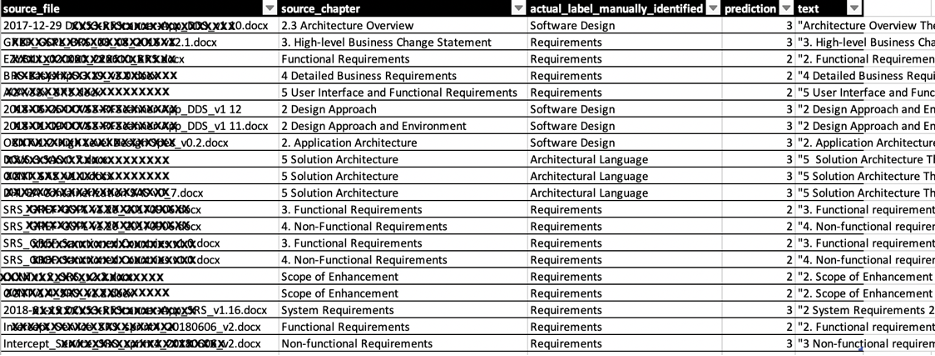
\includegraphics[scale=0.95]{content/pics/Picture_20.png}
\caption{Struktur der Daten, die für Evaluation in diesem Abschnitt genutzt wurden (geschwärzt und gekürzt)}
\label{Abbildung:test-setup}
\end{figure}

{\bf Kriterium 2: Generelle Einsetzbarkeit des Ansatzes im APM-Kontext, unter der Annahme einer beliebig großen Datenmenge}

Wie der Code im Anhang dieser Arbeit zeigt, arbeitet der Ansatz unüberwacht. Das bedeutet, dass auch größere Textmengen für die Erstellung des Modells genutzt werden könnten. Da bereits unter Kriterium 1 gezeigt wurde, dass der Ansatz durchaus Themen schätzen kann, wird das auch bei einer beliebig großen Datenmenge möglich sein. Zu beachten ist, dass die Themen sich inhaltlich stark genug voneinander unterscheiden sollten.

{\bf Kriterium 3: Rechenaufwand}

Eine Implementierung des Verfahrens ist gekapselt in der scikit-learn-Funktion NMF, weshalb auf eine detaillierte Algorithmus-Beschreibung verzichtet wird. Das Verfahren zeichnet sich jedoch durch eine polynomiale Komplexität aus. Das bedeutet, dass der Rechenaufwand je nach Parameterwahl bei der Initialisierung des Modells entsprechend stark steigen kann, je nachdem welche Parameter ausgewählt werden. Zu den Parametern zählt sowohl die Anzahl der Themen, sowie die Textmenge, die für die Modellerstellung verwendet wird \cite{scikit1}.

{\bf Kriterium 4: Kosten}

Es wurden für das Trainings des Modells aufgrund der geringen verwendbaren Datenmenge PDF-Dokumente aus dem Internet verwendet. In der Realität müsste ebenfalls eine ausreichende Trainingsdatenmenge bereitgestellt werden. Dafür sind Texte zusammenzutragen, und es ist insbesondere auf die Qualität der Texte zu achten. Dadurch entstünden Kosten. Kosten für die Nutzung des Verfahrens, z. B. unter Verwendung von Bibliotheken wie scikit-learn \cite{scikit-license}, ergeben sich zunächst nicht.

\section{Ergebnisse: Automatisierte Erzeugung von Text-Zusammenfassungen}

In Abschnitt 3.3 wird begründet, was unter den Ansätzen zur Erzeugung von Text-Zusammenfassungen verstanden wird und wofür sie sinnvoll sein können. Nachfolgend evaluiert werden zunächst ein Ansatz auf Basis von TF-IDF (Abschnitt 4.3.1), gefolgt von einem Ansatz auf Transformer-Basis (Abschnitt 4.3.2). 

\subsection{Ansatz 1: Nutzung eines extraktiven Verfahrens auf Basis von TF-IDF}

Vor der Evaluation soll kurz die Funktionsweise dieses Ansatzes skizziert werden. Die Implementierung besteht aus mehreren Schritten. Eine detaillierte Implementierung mit Kommentaren befindet sich in einem Zip-Archiv, dass dieser Arbeit beigelegt wird.

Der gesamte Textkorpus wird in einzelne Sätze aufgeteilt. Das Vorkommen von Wörtern in einzelnen Sätzen wird anschließend gezählt. Daraus kann nun die TF-Metrik berechnet werden, wie im Theorieteil beschrieben. Im Anschluss wird für jeden Begriff berechnet, in wie vielen Dokumenten dieser vorkommt.

Der nächste Schritt besteht in der Multiplikation der beiden Metriken. Sätze aus dem Text, der zusammengefasst werden soll, werden nun ausgewählt. Das geschieht, indem die TF-IDF-Werte der Begriffe innerhalb eines Satzes addiert werden. Dieser Wert wird geteilt durch die Länge des jeweiligen Satzes. Die Sätze mit den höchsten Werten gelten damit als die wichtigsten Sätze des Dokuments. Ein Grenzwert bestimmt letztendlich, welche Sätze in die finale Zusammenfassung übernommen werden.

{\bf Kriterium 1: Einsetzbarkeit des Ansatzes unter den gegebenen Rahmenbedingungen}

Es wurde für diese Evaluation eins der zur Verfügung stehenden Dokumente ausgewählt.
Um die Güte der durch den Ansatz erzeugten Zusammenfassungen objektiv bewerten zu können, werden von Menschen erzeugte Referenz-Zusammenfassungen benötigt. Diese haben in etwa die gleiche Länge wie die Zusammenfassungen, die automatisch generiert wurden. Bei der Erstellung dieser Referenz-Zusammenfassungen wurde darauf geachtet, dass möglichst viele Sätze so wie sie waren übernommen wurden, ohne manuelles Umschreiben. Es stellte sich heraus, dass die Auswahl von aussagekräftigen Sätzen auch für Menschen, die wenige Hintergrundinformationen zu den eigentlichen Inhalten der Dokumente besitzen, bereits eine Herausforderung ist.
 
Eine ideale durch ein Modell erzeugte Zusammenfassung hätte einen F-Score von 1. In diesem Fall entspräche die Zusammenfassung der durch Menschen erzeugten Referenz-Zusammenfassung. Der F-Score kann interpretiert werden als gewichteter Mittelwert von Precision und Recall \cite{scikit2}. Abbildung \ref{Abbildung:rouge-metrics} stellt sehr geringe F-Scores dar. Das zeigt, dass die automatisch generierten Zusammenfassungen recht weit entfernt von Referenz-Zusammenfassungen liegen. Die Entwicklung der Metrik hängt auch mit der Länge von erzeugten Zusammenfassungen zusammen. Die Länge wird stets kleiner bzw. sie geht gegen Null, wenn der verwendete Korpus vergrößert wird.
Referenz-Zusammenfassungen sind von Menschen mit entsprechender Sorgfalt erstellt worden. Diese Sorgfalt kann dem extraktiven Ansatz nicht bescheinigt werden, d. h. die Qualität der extraktiven Zusammenfassungen ist gering.

\begin{figure}[h]
\centering
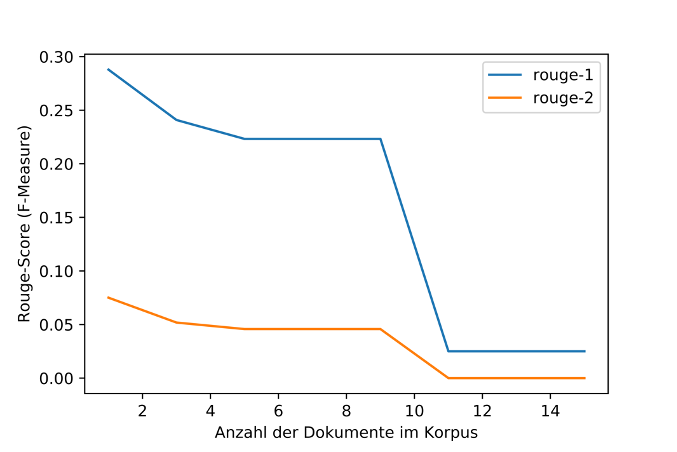
\includegraphics[scale=0.95]{content/pics/Picture_21.png}
\caption{Evaluation der Güte von Zusammenfassungen, unter Veränderung des Ausgangs-Text-Korpus. Eigene Erstellung}
\label{Abbildung:rouge-metrics}
\end{figure}

{\bf Kriterium 2: Generelle Einsetzbarkeit des Ansatzes im APM-Kontext, unter der Annahme einer beliebig großen Datenmenge}

Erwartet wurde zu Beginn, dass bei steigender Datenmenge eine Verbesserung der Rouge-Metrik erreicht werden kann. Wie in Abbildung 21 gezeigt wurde, ist eine solche Tendenz nicht erkennbar.
Eine solche Entwicklung konnte nicht beobachtet werden, weshalb das Verfahren auch bei größeren Datenmengen keine besseren Ergebnisse erbringen wird. 
Wie gezeigt wurde, wird die Güte der Zusammenfassungen von der Größe des Korpus beeinflusst. Die maximale Güte ergibt sich jedoch unter Verwendung von nur einem Text-Dokument als Korpus.

{\bf Kriterium 3: Rechenaufwand}

Dieses Verfahren verwendet eine statistische Herangehensweise und benötigt keine Iterationen oder Ähnliches für die Berechnung der Metriken, die letztendlich bestimmen, welche Sätze in die finale Zusammenfassung aufgenommen werden. Daher kann der notwendige Rechenaufwand vernachlässigt werden, wenn der Textkorpus ausreichend klein gehalten wird.

{\bf Kriterium 4: Kosten}
Wenn davon ausgegangen wird, dass die durch das Verfahren erzeugten Zusammenfassungen sinnvoll genutzt werde könnten, dann würde das Verfahren keine Kosten verursachen, da keine Beschriftungen zu erzeugen sind und Lizenzkosten nicht zu erwarten sind.

\subsection{Ansatz 2: Nutzung eines abstraktiven Verfahrens auf Transformer-Basis}

Im Vergleich zu den extraktiven Verfahren ist das Gebiet der abstraktiven Verfahren zur Erzeugung von Text-Zusammenfassungen eher Gegenstand aktueller Forschung, als eine Klasse von in der Praxis nutzbaren Verfahren \cite[S. 261]{Gupta}. Abbildung \ref{Abbildung:t5} zeigt die erzielten Ergebnisse in einem eigenen Versuch. Evaluiert wird hier das von Google-Forschern entwickelte Modell T5: Text-To-Text-Transfer-Transformer \cite{Raffel}.

\begin{figure}[h]
\centering
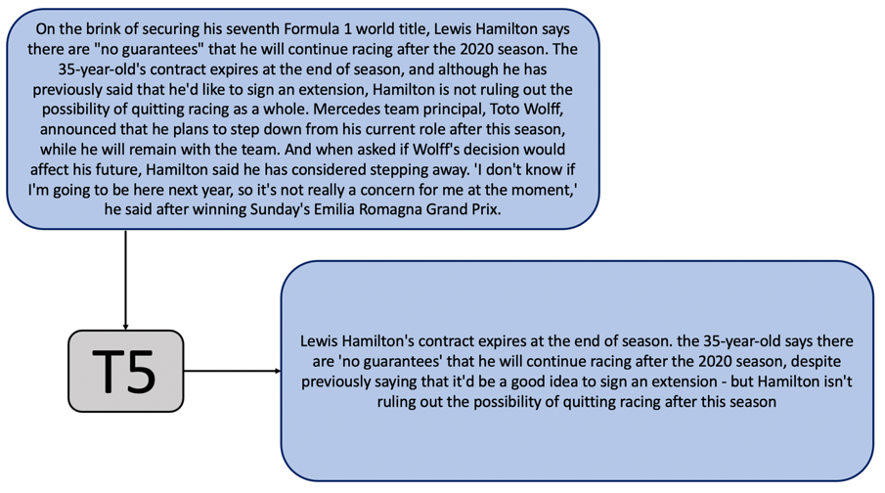
\includegraphics[scale=0.95]{content/pics/Picture_22.png}
\caption{Veranschaulichung eines abstraktiven Verfahrens. Eigene Erstellung in Anlehnung an \cite{Raffel}}
\label{Abbildung:t5}
\end{figure}

{\bf Kriterium 1: Einsetzbarkeit des Ansatzes unter den gegebenen Rahmenbedingungen}

Es ist möglich, ein vorbereitetes Modell  zu verwenden. Auf dieser Grundlage kann eine Fein-Abstimmung durchgeführt werden. Damit könnte erreicht werden, dass das Modell speziell auf Governance-Themen abgestimmt wird. Die Implementierung der Methode wurde im Rahmen der vorliegenden Evaluation in Python realisert. Dafür konnte das Package Transformers (v3.0.2) verwendet werden. Es ermöglicht die Verwendung von vortrainierten Modellen unter dem Slogan ``state-of-the-art NLP for everyone`` \cite{Transformers}.

Es wurden in einer Veröffentlichung CNN/ Daily Mail-Nachrichtentexte unter Verwendung des Modells zusammengefasst und diese Zusammenfassungen wurden mit der Rouge-Metrik evaluiert. Die Ergebnisse dieses Ansatzes setzen neue Maßstäbe bei der Qualität von automatisch generierten Zusammenfassungen \cite[S. 39]{Raffel}. Daher kann gesagt werden, dass die Qualität der Zusammenfassungen als gut eingestuft werden kann, sofern eine Fein-Abstimmung auf den jeweiligen Kontext stattgefunden hat. Die maximale Länge der Eingabe-Sequenz des T5-Modells beträgt nach aktuellem Stand 512 Tokens. Damit können als Eingabe für Zusammenfassungen bislang nur Texte mit maximal 512 Wörtern verwendet werden \cite[S. 39]{Raffel}. Das reicht maximal zur Erzeugung der Zusammenfassung einzelner Abschnitte, die dann kombiniert werden könnten. Das würde jedoch nicht dazu beitragen, dass die wichtigsten Informationen aus einem Text extrahiert werden, was hier eigentlich angestrebt werden sollte.

Longformer (The Long-Document Transformer) ist ein Transformer-Ansatz, der als Alternative zum T5-Modell in Frage käme. Hier wird kontinuierlich versucht die maximale Sequenzlänge der Eingabe zu erhöhen, dennoch gibt es auch hier derzeit noch Beschränkungen auf 4096 Tokens als Eingabe-Sequenz \cite{Longformer} \cite{Longformer2}, was ebenfalls als nicht ausreichend beurteilt werden muss.

Als Fazit wird festgehalten, dass sich die Ansätze noch zu sehr im Entwicklungsstadium befinden und durch die Beschränkung auf sehr kleine Eingabesequenzen keine sinnvollen Ergebnisse im vorliegenden Kontext erzielt werden können. Die notwendige Datenmenge für eine Feinabstimmung wird nachfolgend erläutert. Vorweggenommen werden soll, dass 20-40 Textdokumente dafür nicht ausreichend sind. Unter den gegebenen Rahmenbedingungen ist dieses abstraktive Verfahren also nicht sinnvoll einsetzbar.

{\bf Kriterium 2: Generelle Einsetzbarkeit des Ansatzes im APM-Kontext, unter der Annahme einer beliebig großen Datenmenge}

Wie in Abbildung \ref{Abbildung:t5} verdeutlicht wird, sind grundsätzlich Zusammenfassungen generierbar. Auch im Kontext der IT-Governance geht das, wobei das oben dargestellte Beispiel nur zur Verdeutlichung des Ansatzes dient. Bei der Erstellung des vortrainierten Modells wurde mit dem Colossal Clean Crawled Corpus (C4) eine Datenmenge verwendet, die aus hunderten Gigabytes bereinigten Text aus dem Internet besteht \cite[S. 5-7]{Raffel}. Bei Texten aus dem Internet ist davon auszugehen, dass diese anders zusammengesetzt sind als die Software- oder Architektur-Dokumentationen, um die es im vorliegenden Kontext geht. Daher ist ein solches vortrainiertes Modell noch nicht abgestimmt für den Anwendungsfall. Es sind für eine Fein-Abstimmung entsprechend viele Trainingsdaten notwendig. In einer Veröffentlichung wurde die Fein-Abstimmung auf Basis des CNN-Daily Mail-Datensatzes durchgeführt \cite[S. 37]{Raffel}. Die Größe dieses Datensatzes liegt bei 1.27 Gigabytes. Mit einer solchen Größe ließen sich, wie unter Kriterium 1 bereits beschrieben wurde, auch im APM-Kontext hochwertige Zusammenfassungen erzeugen, allerdings mit der Beschränkung auf 512 Tokens als Eingabesequenz.

Die Fein-Abstimmung ist insbesondere von Bedeutung, weil IT-Dokumentationen in unterschiedlichen Regionen der Welt geschrieben worden sein können. Grammatikalische Regeln werden daher nicht immer eingehalten und Formulierungen können durch lokale Besonderheiten geprägt sein. Vortrainierte Sprachmodelle allein sind daher weniger geeignet, um sinnvolle Zusammenfassungen aus den Dokumentationen zu erzeugen. Ein weiteres Hindernis stellen Abbildungen dar, auf die in den Text-Dokumenten nicht ausreichend eingegangen wird – sie enthalten häufig wichtige Informationen, die durch NLP-Verfahren alleine nicht berücksichtigt werden können. Es müssten zusätzlich weitere ML-Ansätze zur Bildverarbeitung angewendet werden, um optimale Ergebnisse erzielen zu können. Zusammengefasst könnte mit entsprechendem Aufwand eine Feinabstimmung erreicht werden, aufgrund der Beschränkung auf 512 Tokens ist der Ansatz der hier untersucht wurde jedoch (noch) nicht für das APM geeignet.

{\bf Kriterium 3: Rechenaufwand}

Die Zusammenfassungs-Funktionalitäten können unter Verwendung der Bibliotheken direkt genutzt werden, dann allerdings zunächst ohne Fein-Abstimmung. Diese Inferenz dauert auf gängiger Hardware wenige Sekunden, wie beispielhafter Code zeigt, der im Anhang der Arbeit zu finden ist. Versuche der T5-Autoren deuten darauf hin, dass mit mindestens einigen Stunden für die Feinabstimmung zu rechnen ist \cite{Raffel}.

{\bf Kriterium 4: Kosten}

Die Modelle (z. B. t5-small \cite{t5}) sowie die Transformer-Bibliothek \cite{Transformers} sind frei verfügbar. Die vortrainierten Modelle stehen zur Verfügung und können verwendet werden. Nicht zu vernachlässigende Kosten können entstehen durch die Zusammenstellung von Trainingsdaten für die Feinabstimmung eines Modells. Das bedeutet, dass für die Feinabstimmung von Menschen erstellte Zusammenfassungen benötigt werden. Wie beschrieben wurde, kann sich am CNN/ Daily Mail-Beispiel orientiert werden, wo mehrere Gigabytes an Text (Original-Texte + Zusammenfassungen) verwendet wurden. 

\section{Ergebnisse: Automatisierte Schnittstellen-Erkennung}

Die beiden nachfolgenden Ansätze verwenden beschriftete Beispiele für das Training eines Klassifikationsmodells. Die so trainierten Modelle können anschließend genutzt werden, um einzelne Sätze von Textdokumenten in eine der beiden Klassen ``Technisches Interface (TI)`` oder ``kein technisches Interface`` einzuordnen. Wenn die Vorhersage des Modells einem Satz aus der Testmenge die Klasse TI zuteilt, dann kann diese Vorhersage genutzt werden, um Sätze zu identifizieren, in denen eine technische Schnittstelle beschrieben wird. Die Genauigkeit (accuracy) dieser Vorhersage gilt es zu maximieren. Die Qualität und die Menge der Trainingsdaten haben entscheidenden Einfluss auf die Qualität der Vorhersage, wie nachfolgend beschrieben werden soll.

\subsection{Ansatz 1: Klassifizierung auf Grundlage eines BERT-Modells}

BERT, ein vortrainiertes Transformer-Modell, wird hier für die Klassifizierung verwendet, indem das vortrainierte Modell per Fine-Tuning auf den vorliegenden Kontext abgestimmt wird. Dabei werden weitere Schichten eines neuronalen Netzes trainiert, die hinter denen das BERT-Modells liegen, um eine Klassifizierungsaufgabe lösen zu können, wie beschrieben z. B. in \cite[S. 2]{Tang}. Dieser Ansatz heißt Transfer-Learning. Das BERT-Modell kennt bereits grundlegende Eigenschaften von natürlicher Sprache. Es wurde trainiert unter Verwendung des BookCorpus mit 800 Millionen Wörtern sowie der gesamten Englischsprachigen Wikipedia (2500 Millionen Wörter) \cite{devlin}.

{\bf Kriterium 1: Einsetzbarkeit des Ansatzes unter den gegebenen Rahmenbedingungen}

Die für die Feinabstimmung verwendeten Daten setzen sich zusammen aus 195 positiven Beispielen (Klasse TI), und 195 negativen Beispielen (zur Hälfte Sätze zu User Interfaces, zur anderen Hälfte Sätze vollständig ohne Interface-Information). Sie wurden manuell beschriftet. Es werden 70\% der Daten für das Training verwendet, 15\% für das Testen, und 15\% für die Validierung. Die Sätze wurden in einem vorausgegangenen Arbeitsschritt mit einem Ansatz, der auf Ontologien basiert, aus den Textdokumenten des Kunden extrahiert. Der erste Versuch ergab einen f1-score von 70\% (vgl. Abbildung \ref{Abbildung:bert-confusion}). Die interessierende Klasse TI ist erkennbar über die Ausprägung 1. Die Ausprägung 0 gibt an, dass die Vorhersage ``kein TI`` lautete. Die 70\% sind zunächst ein Zeichen dafür, dass Overfitting hier nicht unbedingt ein Problem darstellt. Bei einer verdächtig hohen Genauigkeit müsste davon ausgegangen werden.
 
\begin{figure}[h]
\centering
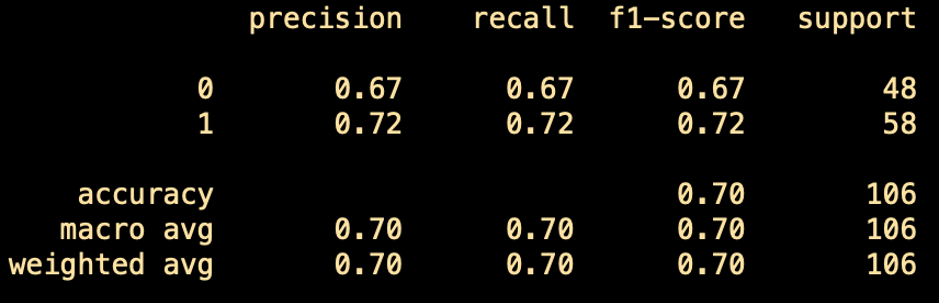
\includegraphics[scale=0.95]{content/pics/Picture_23.png}
\caption{Klassifizierungsergebnisse unter Verwendung von BERT nach der Feinabstimmung. Eigene Bildschirmaufnahme}
\label{Abbildung:bert-confusion}
\end{figure}

Die praktische Einsetzbarkeit in einem realen Szenario bei einer Erkennungsgenauigkeit von (etwa) zwei aus drei Fällen ist fraglich. Angemerkt werden muss, dass sowohl Trainings- als auch Testsätze aus dem gleichen Textkorpus stammen. Zur Folge hätte dies, dass in Produktion, d. h. bei Verwendung eines komplett anderen Dokuments, geschrieben in anderer Art- und Weise, das Modell viel schlechtere Leistung erbringen könnte, als bei den hier vorgestellten Ergebnissen vermutet werden kann. Nachfolgend soll diese Vermutung anhand eines Beispiels evaluiert werden. Es wird eine ``Requirement Specification`` aus dem Internet verwendet, um darin vorkommende Sätze in eine der beiden Klassen (``TI`` oder ``kein TI``) einzuteilen. Interessant ist, dass dieses Verfahren zunächst nicht direkt eine Klasse als Vorhersage ausgibt, sondern zwei Werte. Das sind die direkten Ausgaben des neuronalen Netzes, das für die Klassifizierung verwendet wird. Es wird der absolut größere Wert verwendet für die Bestimmung der Klasse. Eindeutig als ``kein technisches Interface`` (Klasse 0) können damit Sätze bestimmt werden, die offensichtlich kein Interface beschreiben (Abbildung \ref{Abbildung:bert-0}). Bei längeren Sätzen sind in diesem Beispiel allerdings auch viele Sätze dabei, die nichts mit Interfaces zu tun haben, aber als solche klassifiziert wurden (Abbildung \ref{Abbildung:bert-1}).

\begin{figure}[h]
\centering
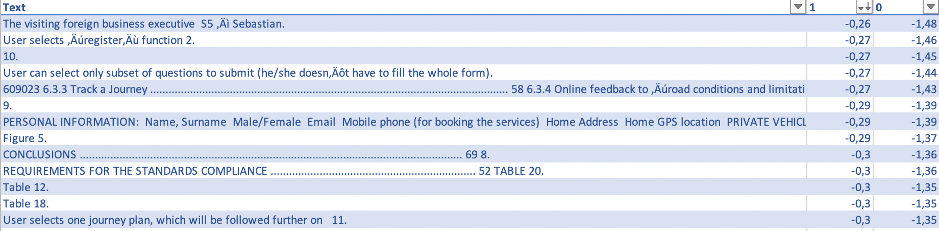
\includegraphics[scale=0.95]{content/pics/Picture_25.png}
\caption{Klasse 0 (``kein TI``) gewinnt und bestimmt damit die Vorhersage. Eigene Bildschirmaufnahme}
\label{Abbildung:bert-0}
\end{figure}

\begin{figure}[h]
\centering
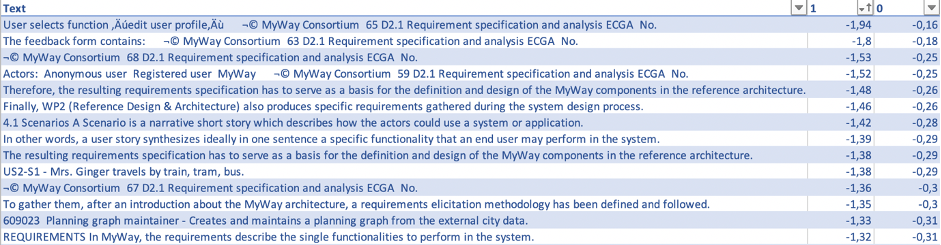
\includegraphics[scale=0.95]{content/pics/Picture_26.png}
\caption{Beispiele, bei denen Klasse 1 als Vorhersage bestimmt wurde. Eigene Bildschirmaufnahme}
\label{Abbildung:bert-1}
\end{figure}

Es wird festgehalten, dass die Feinabstimmung mit der gegebenen Datenmenge nicht ausreichend ist, um in der Praxis mit dem Ansatz sinnvolle Ergebnisse zu erreichen. Die Kernaussage ist aber, dass der Ansatz im Sinne eines Proof-of-Concepts funktionsfähig und in der Perspektive vielversprechend ist.

{\bf Kriterium 2: Generelle Einsetzbarkeit des Ansatzes im APM-Kontext, unter der Annahme einer beliebig großen Datenmenge}

Um die Güte des Verfahrens messen zu können, wären weitere beschriftete Daten notwendig. Diese müssen in ausreichender Qualität vorhanden sein, und am besten durch Experten beschriftet worden sein. Es wäre auch denkbar, dass mehrere Experten die Beschriftungen vergeben und letztendlich nur die Beschriftung für das Training verwendet wird, die von mehreren Personen als Beschriftung ausgewählt wurde. Damit würden Zweifel eliminiert werden, darüber welche Klasse die richtige für einzelne Sätze ist. In anderen Veröffentlichungen wird von Genauigkeiten von bis zu 97\% bei ausreichend großen Datenmengen berichtet \cite{Tang}. Daher wird zusammengefasst, dass dieser Ansatz generell einsetzbar sein könnte, um Schnittstellen in Texten zu identifizieren, allerdings erst dann, wenn beschriftete Trainings-Beispiele in ausreichender Menge vorliegen.

{\bf Kriterium 3: Rechenaufwand}

Es wird lediglich die Fein-Abstimmung eines BERT-Modells durchgeführt. Ein großer Teil der Gewichtungen des Netzes ist also bereits verfügbar und muss nicht erneut berechnet werden \cite{bert}.
Das Training kann auf einer CPU oder auf einer GPU durchgeführt werden\footnote{vgl. Code im Anhang}. Die Dauer der Fein-Abstimmung ist stets abhängig davon welche Prozessorarchitektur verwendet werden kann. Außerdem ist sie von gewählten Hyperparametern (Epochen/ Learning Rate, etc.) abhängig. Auf einer CPU dauert die Feinabstimmung länger als auf einer GPU. Es muss mit einigen Minuten auf gewöhnlicher Hardware kalkuliert werden. Die Inferenz (Vorhersage) nach dem Training ist ohne größere Verzögerungen möglich.

{\bf Kriterium 4: Kosten}

Das Auszeichnen von Sätzen ist der Kostentreiber bei diesem Ansatz. Dieser Aufwand erfolgt bei Einführung des Ansatzes, im Laufe der Zeit können jedoch Anpassungen notwendig werden. Es wäre denkbar, dass mehrere Menschen über die Beschriftungen entscheiden, etwa nach dem Mehrheitsprinzip: es wird die Beschriftung von dem Modell verwendet, für die sich die Mehrheit entschieden hat. Da Kenntnisse auf Expertenniveau benötigt werden, kann dieser Ansatz entsprechende Kosten verursachen. Lizenzkosten sind nicht zu erwarten, da die Apache-2.0-Lizenz verwendet wird \cite{bert}.

\subsection{Ansatz 2: Klassifizierung mit logistischer Regression auf Basis von N-Grammen}

Das Ziel ist hier wie bereits schon in Abschnitt 4.4.1 die Erkennung von Interface-Sätzen. In Kontrast zu dem vorangegangenen Ansatz, der auf Deep Learning sowie dem Transformer-Modell basierte, wird hier nun ein anderer Ansatz untersucht. Dadurch können die Ergebnisse der beiden Klassifizierungs-Ansätze besser eingeschätzt und verglichen werden. 

Es handelt sich bei diesem Ansatz um die Klassifizierung von einzelnen Sätzen mit logistischer Regression. Es wird auf Wort-Vektoren oder ein vortrainiertes Transformer-Modell verzichtet und stattdessen werden aus Texten nur N-Gramme gebildet, die später als Features für die logistische Regression verwendet werden. Es werden die typischen Schritte \cite[S. 124]{Gupta} für eine Klassifizierung verfolgt. Die Implementierung ist überschaubar, weshalb sie anhand des schematischen Programmcodes (Abbildung \ref{Abbildung:lr-code}) beschrieben werden sollen. Der Code ist gekürzt, unter anderem wurden die Importe der Bibliotheken entfernt.

\begin{figure}[h]
\centering
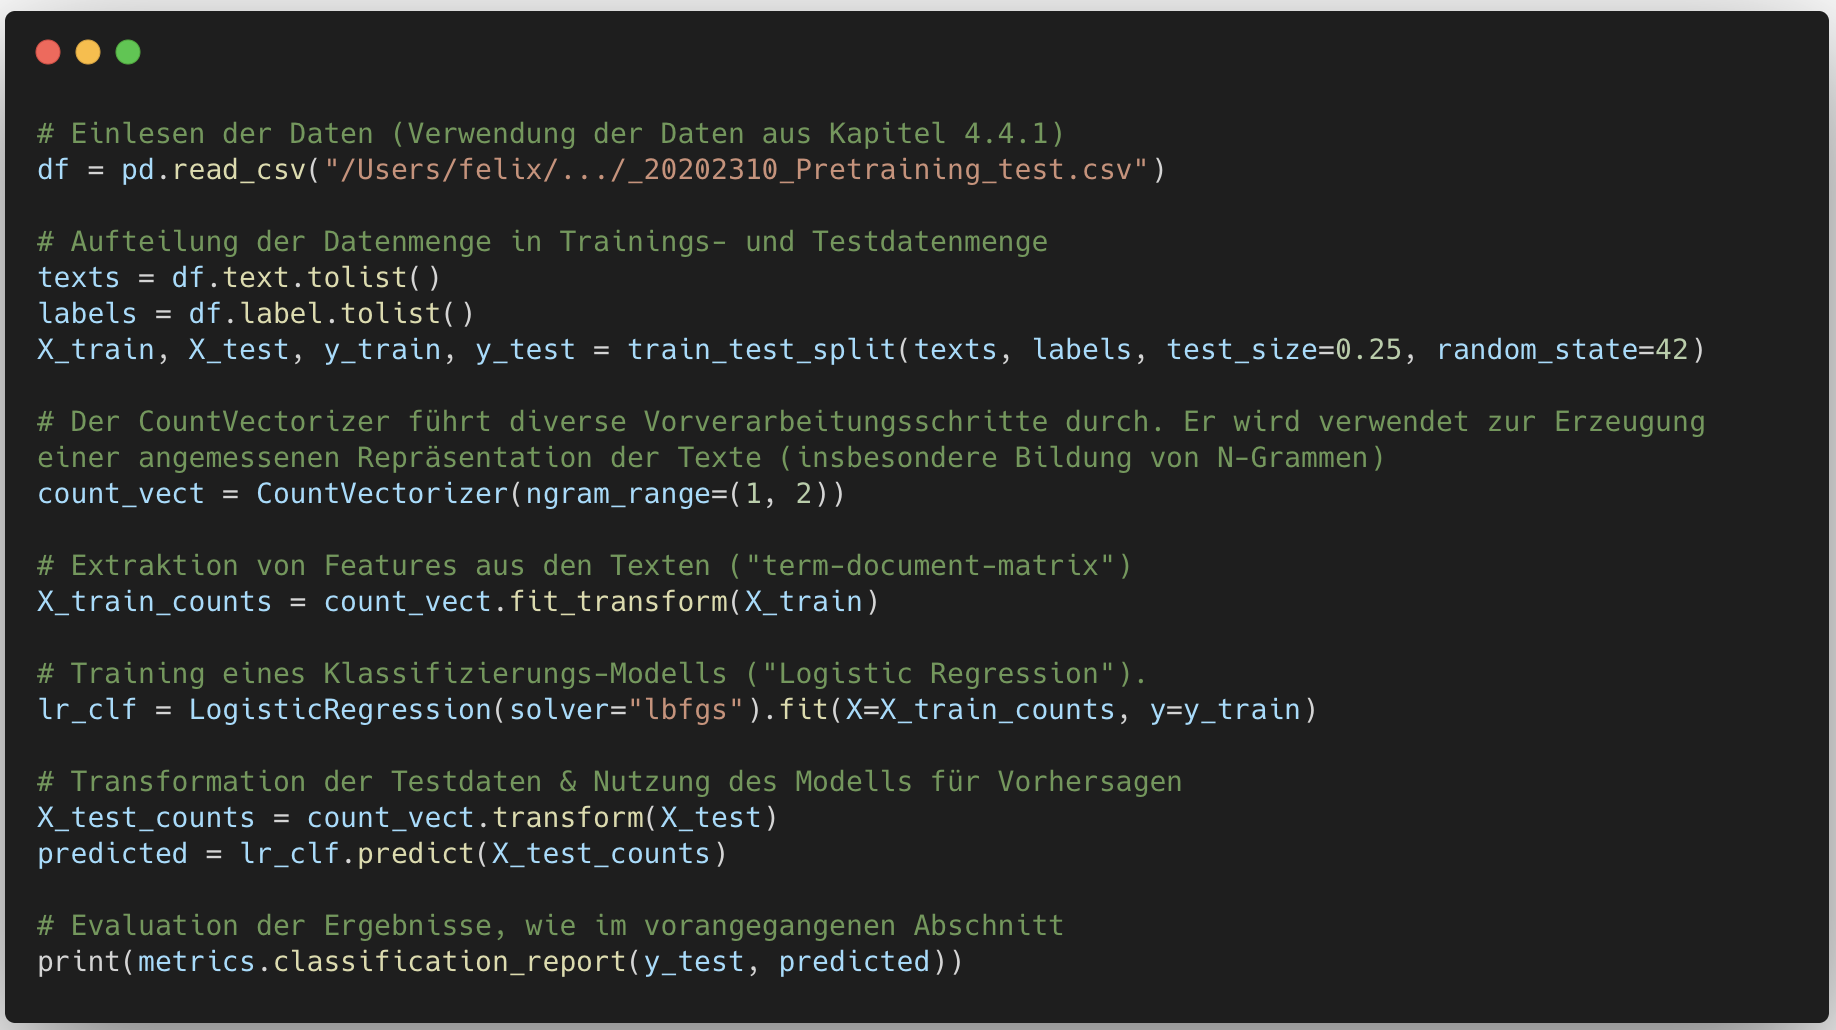
\includegraphics[scale=0.4]{content/pics/Listing_2_.png}
\caption{Klassifizierung mit logistischer Regression. Eigene Erstellung}
\label{Abbildung:lr-code}
\end{figure}

{\bf Kriterium 1: Einsetzbarkeit des Ansatzes unter den gegebenen Rahmenbedingungen}

Es werden nachfolgend in \ref{Abbildung:lr-test} die Ergebnisse des Versuchs aus \ref{Abbildung:lr-code} präsentiert.

\begin{figure}[h]
\centering
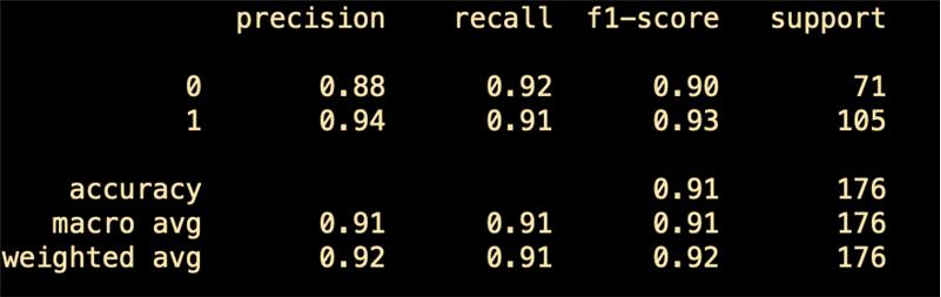
\includegraphics[scale=0.95]{content/pics/Picture_27.png}
\caption{Ergebnisse der Klassifizierung von Sätzen aus der Testmenge. Eigene Bildschirmaufnahme}
\label{Abbildung:lr-test}
\end{figure}

Diese zunächst gutaussehenden Ergebnisse können wohl durch Overfitting erklärt werden. Dieser Umstand ist der geringen Datenmenge geschuldet. Ein Versuch mit einem komplett anderen Dokument (vgl. \ref{Abbildung:lr-eval}) etwa klassifiziert 153 der insgesamt 494 Sätze aus diesem Dokument in die TI-Klasse (entspricht Klasse 1 in \ref{Abbildung:lr-eval}; es geht um das gleiche Dokument bzw. das gleiche Vorgehen wie in 4.4.1). Zu sehen ist, dass Sätze in Klasse 0 (``kein technisches Interface``) tatsächlich häufig korrekt klassifiziert wurden. Genauso häufig werden aber auch Sätze, die offensichtlich nichts mit Interfaces zu tun haben, in Klasse 1 (technisches Interface) klassifiziert, was nicht korrekt ist.

\begin{figure}[h]
\centering
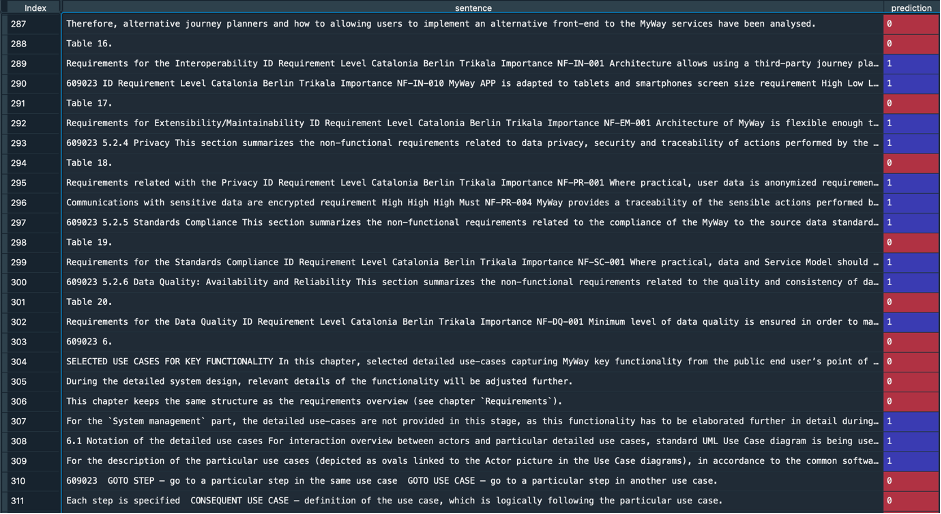
\includegraphics[scale=0.95]{content/pics/Picture_28.png}
\caption{Einige Vorhersagen für ein Evaluations-Dokument. Eigene Bildschirmaufnahme}
\label{Abbildung:lr-eval}
\end{figure}

Deshalb kann die produktive Einsetzbarkeit des Verfahrens unter den gegebenen Rahmenbedingungen mit relativ wenigen Datensätzen für das Training eines Modells nicht bestätigt werden.

{\bf Kriterium 2: Generelle Einsetzbarkeit des Ansatzes im APM-Kontext, unter der Annahme einer beliebig großen Datenmenge}

Hier \cite{Vogelsang} wurde eine ähnliche Klassifikation durchgeführt. Die Autoren verwendeten 89 Text-Dokumente für das Training des Klassifikationsmodells. Erreicht wurde, dass 4 von 5 Test-Dokumenten korrekt klassifiziert wurden – ein grundsätzlich gutes Ergebnis, erreicht mit einer kleinen Trainingsmenge. Es kann jedoch gesagt werden, dass bei steigenden Trainingsdatenmengen recht zuverlässige Ergebnisse erzielt werden können, was auch für den vorliegenden Kontext gelten würde. Damit kommt das Verfahren bei ausreichender Trainingsdatenmenge durchaus für den Einsatz in Frage. 

{\bf Kriterium 3: Rechenaufwand}

Die Vorverarbeitung, sowie das Training des Modells erfolgen in wenigen Sekunden. Die Anwendung zur Vorhersage von neuen Datensätzen erfolgt ebenfalls in wenigen Sekunden.

{\bf Kriterium 4: Kosten}

scikit-learn kann kostenfrei genutzt werden \cite{scikit-license}. Zur Verbesserung und Weiterentwicklung des Modells müssen weitere Sätze beschriftet und weitere Dokumente gesammelt werden. Das erzeugt manuellen Aufwand.

\section{Zusammenfassung der Ergebnisse}

Dieser Abschnitt stellt die Ergebnisse der Evaluation zusammenfassend in einer Übersicht dar. Des Weiteren enthält Tabelle \ref{tab:zusammenfassung} eine Handlungsempfehlung zum weiteren Vorgehen mit den Verfahren.


% Please add the following required packages to your document preamble:
% \usepackage{multirow}
\begin{table}[h]
\centering
\begin{tabular}{|c|c|c|}
\hline
\textbf{Kategorie}                                                                                                & \textbf{Ansatz}                                                                                              & \textbf{\begin{tabular}[c]{@{}c@{}}Handlungsempfehlung/ \\ Zusammenfassung\end{tabular}}                                          \\ \hline
\multirow{2}{*}{\begin{tabular}[c]{@{}c@{}}Ermittlung \\ von \\ Ähnlichkeiten\end{tabular}}                       & \begin{tabular}[c]{@{}c@{}}Mit einem (vortrainierten) \\ Word2Vec-Modell\end{tabular}                        & \begin{tabular}[c]{@{}c@{}}Gute Grundlage. \\ Weiterentwicklung \\ kann sinnvoll sein.\end{tabular}                               \\ \cline{2-3} 
                                                                                                                  & \begin{tabular}[c]{@{}c@{}}Unter Verwendung des \\ Paragraph-Vector-Modells (Doc2Vec)\end{tabular}           & \begin{tabular}[c]{@{}c@{}}Kann bei ausreichenden\\ Datenmengen sinnvoll sein.\\ Weiterentwickeln.\end{tabular}                   \\ \hline
\multirow{2}{*}{\begin{tabular}[c]{@{}c@{}}Bestimmung von \\ inhaltlicher \\ Integrität\end{tabular}}             & \begin{tabular}[c]{@{}c@{}}Durch Erzeugung und den Vergleich \\ von Durchschnitts-Wort-Vektoren\end{tabular} & \begin{tabular}[c]{@{}c@{}}Ist höchstens sinnvoll, \\ um absolut unpassende Texte \\ (``lorem ipsum``) zu entdecken.\end{tabular} \\ \cline{2-3} 
                                                                                                                  & Mit Topic Modeling (NMF)                                                                                     & \begin{tabular}[c]{@{}c@{}}Gute Grundlage. \\ Weiterentwicklung \\ kann sinnvoll sein.\end{tabular}                               \\ \hline
\multirow{2}{*}{\begin{tabular}[c]{@{}c@{}}Automatisierte \\ Erzeugung \\ von Zusammen-\\ fassungen\end{tabular}} & \begin{tabular}[c]{@{}c@{}}Mit einem \\ extraktiven Ansatz (TF-IDF)\end{tabular}                             & \begin{tabular}[c]{@{}c@{}}Nicht sinnvoll.\\ Idee verwerfen.\end{tabular}                                                         \\ \cline{2-3} 
                                                                                                                  & \begin{tabular}[c]{@{}c@{}}Mit einem \\ abstraktiven Ansatz (T5)\end{tabular}                                & \begin{tabular}[c]{@{}c@{}}Noch nicht \\ sinnvoll einsetzbar. \\ Weiter beobachten\end{tabular}                                   \\ \hline
\multirow{2}{*}{\begin{tabular}[c]{@{}c@{}}Automatisierte\\ Schnittstellen-\\ erkennung\end{tabular}}             & \begin{tabular}[c]{@{}c@{}}Per Klassifizierung von Sätzen \\ mit BERT und einem neuronalen Netz\end{tabular} & \begin{tabular}[c]{@{}c@{}}Weiter beobachten. \\ Weitere Trainingsdaten \\ anlegen und weiterentwickeln.\end{tabular}             \\ \cline{2-3} 
                                                                                                                  & \begin{tabular}[c]{@{}c@{}}Per Klassifizierung von Sätzen \\ mit logistischer Regression\end{tabular}        & \begin{tabular}[c]{@{}c@{}}Weiterentwickeln, insbesondere \\ um eine Referenz zu anderen\\  Ansätzen zu erhalten.\end{tabular}    \\ \hline
\end{tabular}
\caption{Zusammenfassung der Evaluations-Ergebnisse}
\label{tab:zusammenfassung}
\end{table}

%add more chapters


\cleardoublepage
\clearpage


%%%%%%%%%%%%%%%%%%%%%%%%%%%%%%%%%END - Content

\singlespacing
\pagenumbering{roman}   % i, ii, iii, iv, ...
\setcounter{page}{1}

\nocite{*}
\printbibliography

%\printbibliography[title={Title of online sources}, type=online]

\cleardoublepage
\chapter*{Eidesstattliche Versicherung}
\addcontentsline{toc}{chapter}{Eidesstattliche Versicherung}  
What you want..
\chapter*{Anhang}
\addcontentsline{toc}{chapter}{Anhang}  
Der Python-Code, der für die in dieser Arbeit beschriebenen Evaluationen verwendet wurde, ist in einem Zip-Archiv zu finden, das mit der Ausarbeitung abgegeben wird.  

\end{document}
